\documentclass[11pt,a4paper, fleqn]{article}
\usepackage{amsmath,europs,booktabs,amssymb,bm,soul}
%\usepackage[euler-digits,euler-hat-accent]{eulervm}
\usepackage{mathpazo}
\usepackage[T1]{fontenc}
\usepackage{baskervald}%\usepackage{lmodern}
%\usepackage[T1]{fontenc}
%\usepackage{tgheros}
%\renewcommand{\familydefault}{\sfdefault} 
\usepackage{float}
\usepackage{url}
\usepackage{eurosym}
\usepackage[right=2.8cm,left=2.8cm,top=3.2cm,bottom=2.8cm]{geometry}
\usepackage[FIGBOTCAP]{subfigure}
\usepackage[english]{babel} %LANGUAGE
%\usepackage{ucs} 
\usepackage[utf8]{inputenc}
\usepackage[usenames,dvipsnames]{color}
\usepackage{graphicx}
\usepackage{chngpage}
%\usepackage{cite}
\usepackage{appendix}
\usepackage[hang,small,bf,figurewithin=section,tablewithin=section]{caption}
\usepackage{rotating}
\usepackage{caption}
\usepackage{picins}
\usepackage{array}
\usepackage{wrapfig}
\usepackage{xspace}
\usepackage[absolute]{textpos}
\usepackage{hyperref}
\usepackage[hyphenbreaks]{breakurl}
\usepackage[table]{xcolor}
\setlength{\TPHorizModule}{1mm}
\setlength{\TPVertModule}{\TPHorizModule}
\definecolor{myblue}{rgb}{0,0,0.4}
\definecolor{gray}{rgb}{0.5,0.5,0.5}
\usepackage{listings}
\setlength{\parskip}{0.1ex}
\setlength{\parindent}{0mm}
\newcommand{\degree}{\ensuremath{^{\circ}}\xspace}
\newcommand{\HRule}{\rule{--\linewidth}{0.5mm}}
%\numberwithin{equation}{section}
%\numberwithin{figure}{section}
%\numberwithin{table}{section}
\definecolor{dkgreen}{rgb}{0,0.6,0}
\definecolor{gray}{rgb}{0.5,0.5,0.5}
\definecolor{mauve}{rgb}{0.58,0,0.82}
\usepackage{fancyhdr}
\usepackage{graphicx} % To be able to edit graphics
\usepackage{caption}
\usepackage{xfrac}
\usepackage{longtable}
\usepackage[nottoc]{tocbibind}
\usepackage[makeroom]{cancel}
\usepackage[style=ieee,sorting=nyt]{biblatex}
\usepackage{mhchem}
\usepackage{siunitx}
\usepackage[framed,numbered,autolinebreaks,useliterate]{mcode}
\usepackage{inconsolata}

%\usepackage{draftwatermark} %Watermark
\newcommand{\tightoverset}[2]{\mathop{#2}\limits^{\vbox to -.5ex{\kern-0.75ex\hbox{$#1$}\vss}}}
  
\lstset{breaklines=true,
  basicstyle=\ttfamily,
  columns=fullflexible,
  frame=single,
  breaklines=true,
  language=Matlab}

%\lstset{
%  basicstyle=\ttfamily,
%  columns=fullflexible,
%  frame=single,
%  breaklines=true,
%  language=Matlab
%}
\pagestyle{fancy}
\renewcommand{\sectionmark}[1]{\markboth{#1}{}}
\renewcommand{\subsectionmark}[1]{\markright{\thesection\ #1}{}}
\fancyhead{}
%\fancyfoot{}
\renewcommand{\headrulewidth}{0pt}
\renewcommand{\footrulewidth}{0pt}
%\lhead{\small \thepage}
\rfoot{\small T.M.J. Bouts}
\lfoot{\small 4BM40}
\cfoot{\small \thepage}

\begin{document}
\setcounter{page}{1}
\pagenumbering{arabic}
\vspace*{-2.5cm}
\begin{center}
\large{\textsf{4BM40 \\
Optical diagnostics for combustion and fluid flow \\
T.M.J. Bouts - 0904096\\
\today}}
\section*{Assignment 1}
\setcounter{section}{1}
\setcounter{subsection}{1}
\end{center}
\subsubsection{}
First a plot is created by choosing `Linear Molecule' in PGOPHER.
\begin{figure}[H] 
\centering
\includegraphics[scale=2]{figure.png}
\caption{Linear Molecule from PGOPHER displaying the rovibrational spectrum}
\label{Figure}
\end{figure}
To determine which of the curves is the P-branch and which one is the R-branch, the energy exchange has to be analysed. There is no Q-branch in this case. Assuming that the electronic state doesn't change, the energy exchange can be written down as:
\begin{equation} \label{energy}
	\Delta E = \omega_e \left(\nu_i - \nu_f \right)+B_i J_i (J_i +1)-B_f J_f (J_f +1)
\end{equation}
where $i$ mean initial and $f$ means final. A couple of assumptions have been made, namely $\left(\nu_i - \nu_f \right) = 1$ and $B_i = B_f$. If the P-branch is used, $J_f = J_i -1$ and if the R-branch is used, $J_f = J_i +1$. When we substitute $J_f$ of the P-branch in \eqref{energy}, 
\begin{equation}
	\Delta E = \omega_e +B_i J_i (J_i +1)-B_i (J_i -1) \cdot (J_i -1 +1) 
\end{equation}
can be created. Which in turn results in:
\begin{equation}
	\Delta E = \omega_e +B_i J_i \left[ (J_i +1)-(J_i -1) \right] = \omega_e +2 B_i J_i
\end{equation}
which shows that $\Delta E$ will be increased when the P-branch is selected. For the R-branch a similar derivation can be done. Here we substitute $J_f = J_i + 1$ in \eqref{energy}, this results in:
\begin{equation}
	\Delta E = \omega_e +B_i J_i (J_i +1)-B_i (J_i + 1) \cdot (J_i + 1 +1)
\end{equation}
which again can be rewritten into:
\begin{equation}
	\Delta E = \omega_e +B_i (J_i +1) \left[ J_i - (J_i +2) \right] = \omega_e -2 B_i (J_i +1)
\end{equation}
which shows that $\Delta E$ decreases for the R-branch. 
To determine which peak belongs to which branch, 
\begin{equation} \label{Delta}
\Delta E = \frac{h c}{\lambda_{in} - \lambda_{out}} \equiv \bar{\nu}_{in} - \bar{\nu}_{out}
\end{equation}
will be used. Rewriting \eqref{Delta} results into:
\begin{equation}
	\bar{\nu}_{out} = \bar{\nu}_{in} -\Delta E
\end{equation}
Using the fact that $\Delta E$ increases for the P-branch, it can be determined that $\bar{\nu}_{out}$ decreases and therefore must be the left peak in Figure \ref{Figure}. For the R-branch $\Delta E$ decreases and therefore gets a higher $\bar{\nu}_{out}$ and must be the right peak in Figure \ref{Figure}. If we zoom in a little on the middle part of the graph at around 1000 \si{\per\cm}, it will be easier to assign the rotational quantum numbers. 
\begin{figure}[H]
	\centering 
	\includegraphics[scale=2]{fig2.png}
	\caption{Rotational quantum numbers $J$ around 1000 \si{\per\cm} of the spectrum}
\end{figure} 

The maximum rotational quantum number is $J\approx10$ in this case. This number $10$ is assigned to the peaks in the spectrum. If we start counting back we can see that the left peak close to 1000 \si{\per\cm} is equal to 1 and the right peak close to 1000 \si{\per\cm} is equal to 0. There is no line at the central line (1000 \si{\per \cm}) because the Q-branch is not allowed ($\Delta J \pm 1$ and $\Delta E = \omega_e$); the quantum numbers must change. The shape of the graph is a distance of $2B$ between every $J$ except for the peaks right and left of 1000 \si{\per\cm}, here the peaks have a distance of $4B$. Furthermore is the intensity  proportional to the amount of molecules that have made the changeover. The quantum numbers can also more easily be seen in a `Fortrat Diagram'.

\subsubsection{}  
Nothing happens, an empty plot figure is created. The two options state:
\begin{itemize}
\item Symmetry: Set true if the molecule has a centre of symmetry, and g or u must be specified for individual states 
\item  SymWt: statistical weight of symmetric rotational levels, or all levels if no centre of symmetry 
\end{itemize} 
Here `Symmetry' is set to \textit{True}. This means that the molecule has a center of symmetry. `SymWt' is set to 0. Therefore the statistical weight of symmetric rotational levels is 0. Hence the empty plot.

\subsubsection{}  \label{ch3}
The plots are located in the Appendix \ref{Appendix}. The B value has been increased in steps of 0.01 in the excited state. In the left part of the graph, the lines move more to the right and get closer together. It may be caused by the effect the $B_f$ in \eqref{energy} is increased, and therefore $\Delta E$ is decreased. So it will get a higher $\nu _{out}$, which results in a shift to the right. I would expect that the right curve shows similar behaviour. So the lines will move closer and further to the left. After doing a test by decreasing $B$ to $0.9$, it does move further to the left and closer together. 
 
\subsubsection{}
`Band head' happens when the lines in the branch pile up and the branch reverses direction. For the P-branch the first order P-line frequencies are given by
\begin{equation}
	\bar{\nu}(J) = \Delta E_{rot} = -(B_e' + B_e'')J+(B_e'-B_e'')J^2
\end{equation}
where $B_e' = B_1$, $B_e'' = B_0$ can be rewritten to
\begin{equation*}
\frac{\bar{\nu}(J)}{J} + (B_1 + B_0) = (B_1-B_0)J 
\end{equation*}
\begin{equation*}
J = \frac{\bar{\nu}(J)}{J\cdot(B_1-B_0)}+ \frac{(B_1 + B_0)}{(B_1-B_0)}
\end{equation*}
\begin{equation*}
J = \frac{\bar{\nu}(J)}{J\cdot(B_1-B_0)}+ \frac{B_1}{(B_1-B_0)}+ \frac{B_0}{(B_1-B_0)}
\end{equation*}
\begin{equation}
	J \approx \frac{B_0}{(B_1-B_0)}
\end{equation}
\subsubsection{}
As seen in Figure \ref{fig:lorgau}, the first thing that's changed by increasing `Gau' or `Lor' is that the bars are now connected in so they form wave like structures. Another things that should be noticed is that the intensity is changed, especially by changing the `Lor' value. The Lorentzian lowers the intensity and decreases the slope. The lifetime is limited due to spontaneous emission and the Lorentzian includes this natural lifetime. The Gaussian value includes `Doppler broadening'. The velocity is linear with the perceived frequencies, the frequencies get the same form. Since the molecules that absorb a certain frequency are proportional to the absorption coefficient, this takes on the same form as well.
\begin{center}
	\begin{minipage}{\linewidth}
		\begin{minipage}{0.5\linewidth}
			\begin{figure}[H]
				\centering 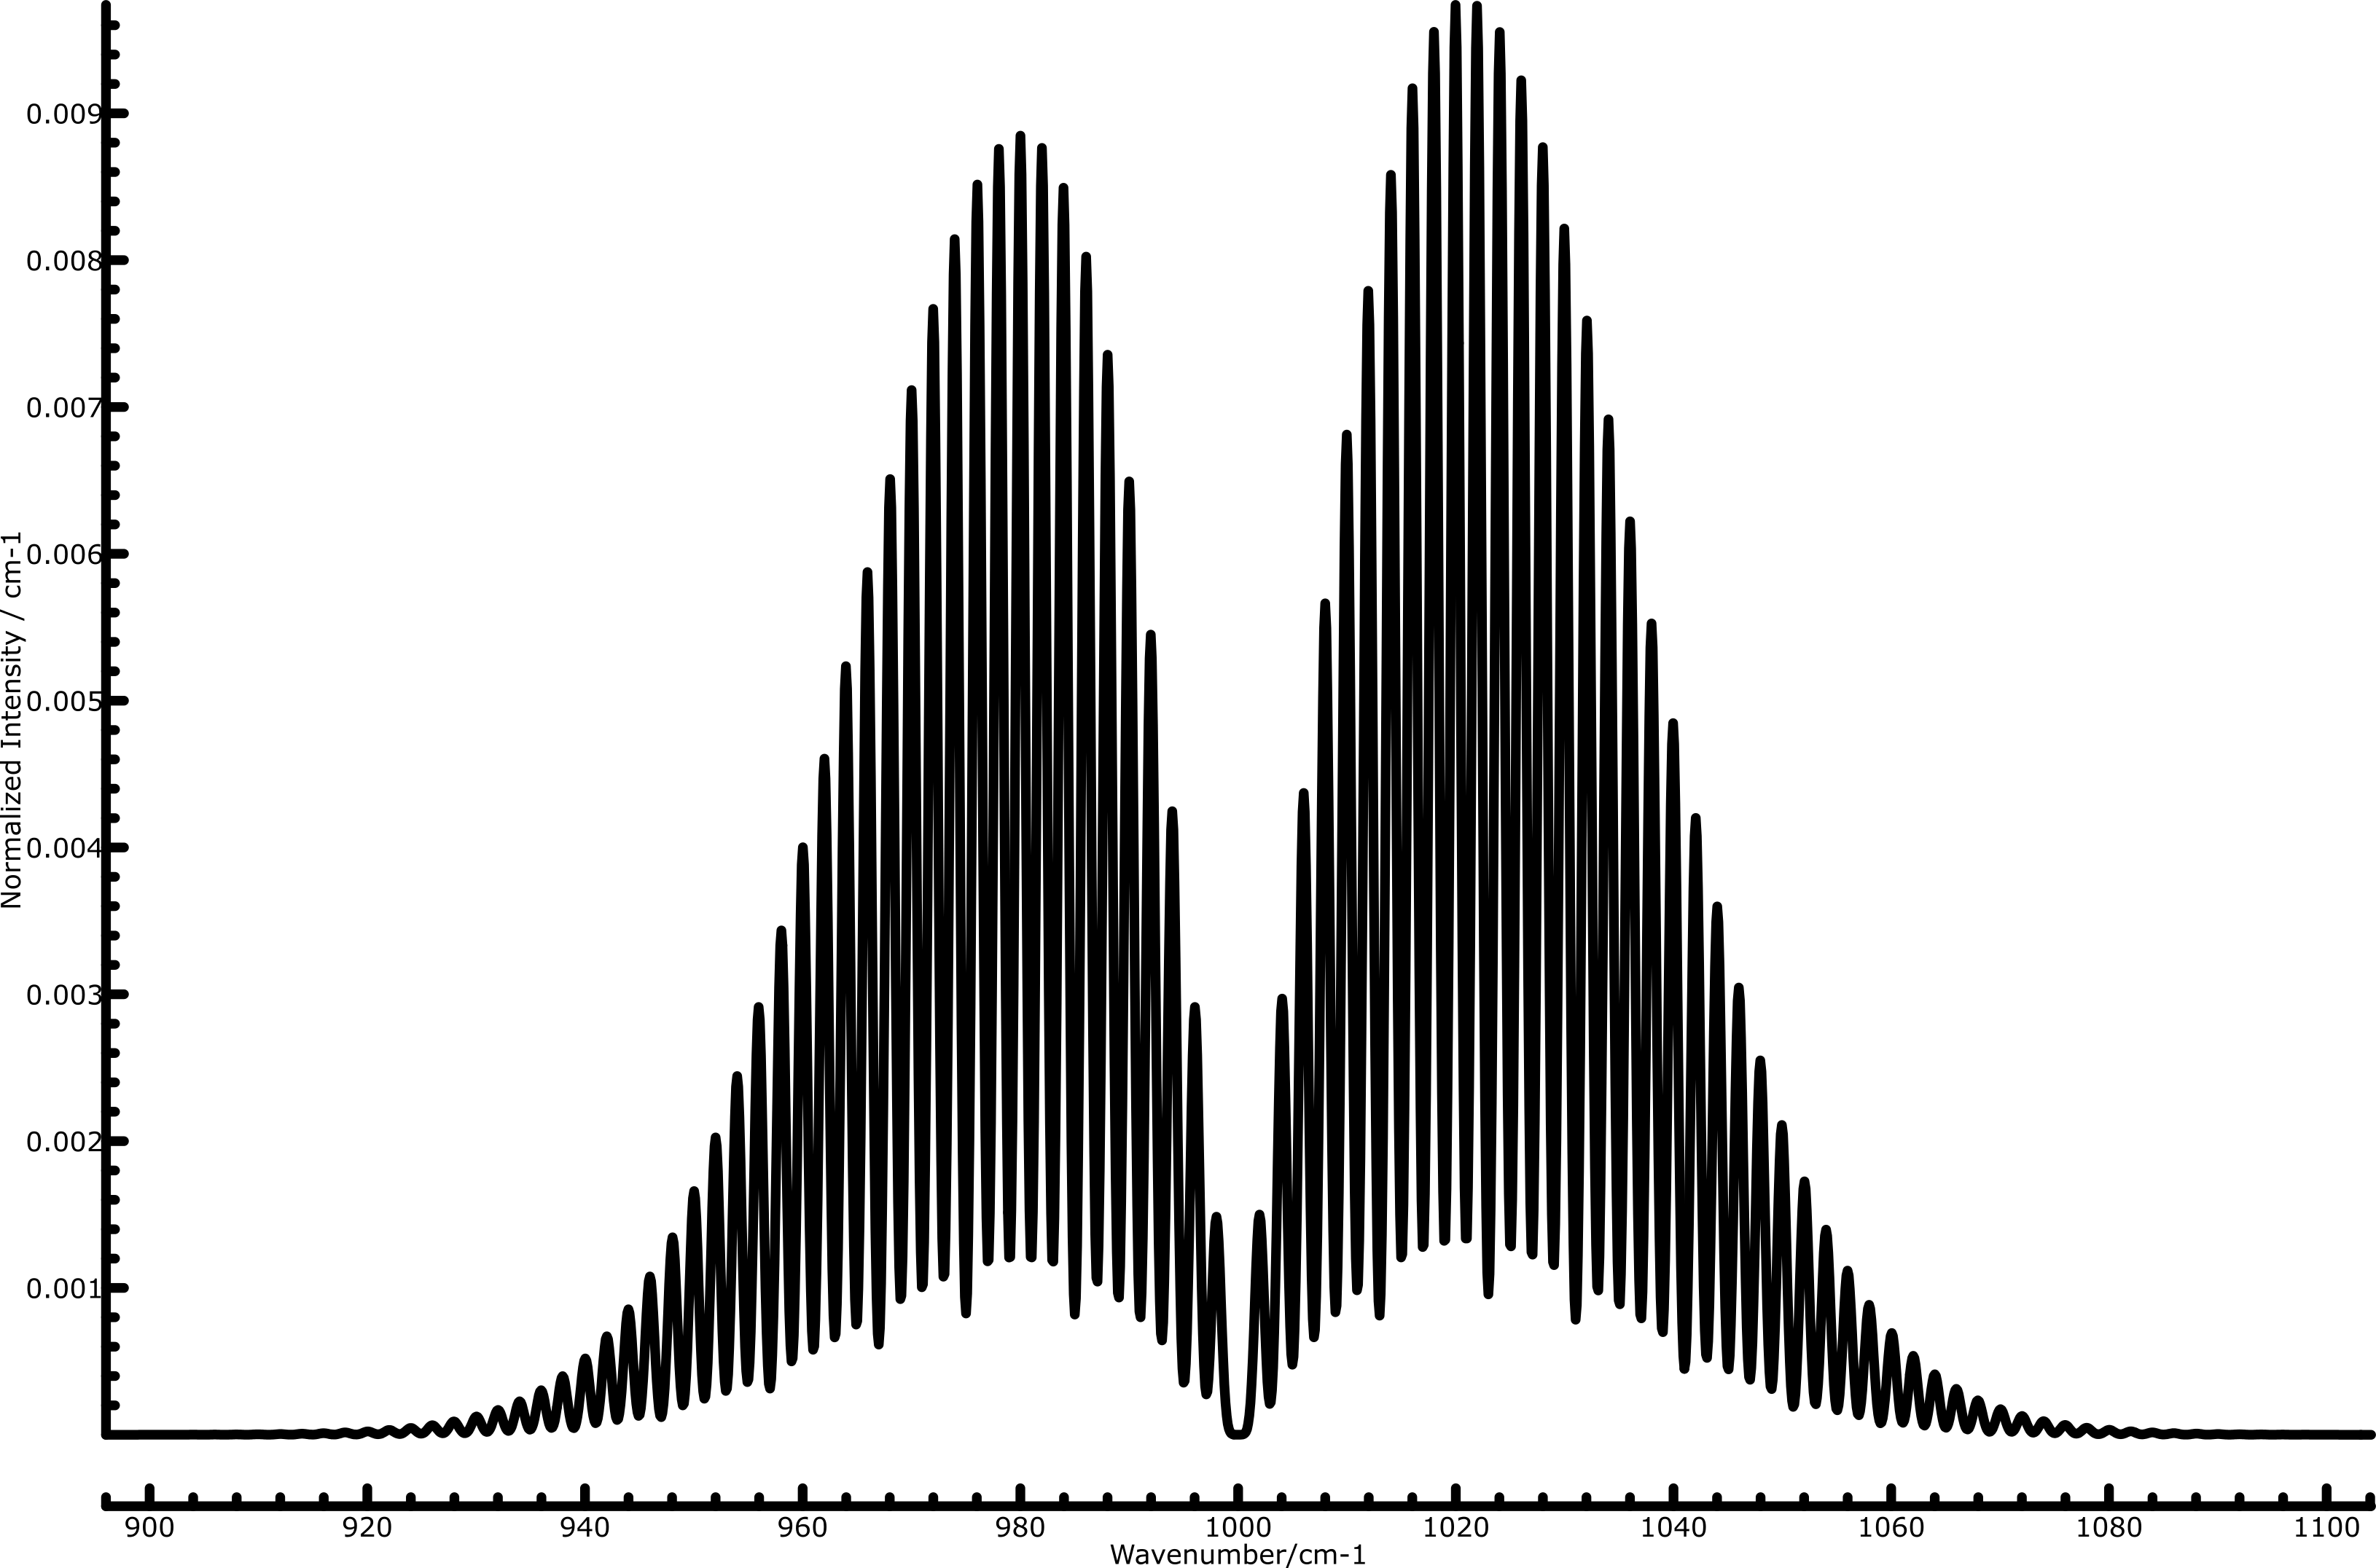
\includegraphics[width=\linewidth] 						{figures/Gau1.png}
			\end{figure} 
				\centering(a) \\
		\end{minipage}
		\begin{minipage}{0.5\linewidth}
		   \begin{figure}[H]
				\centering 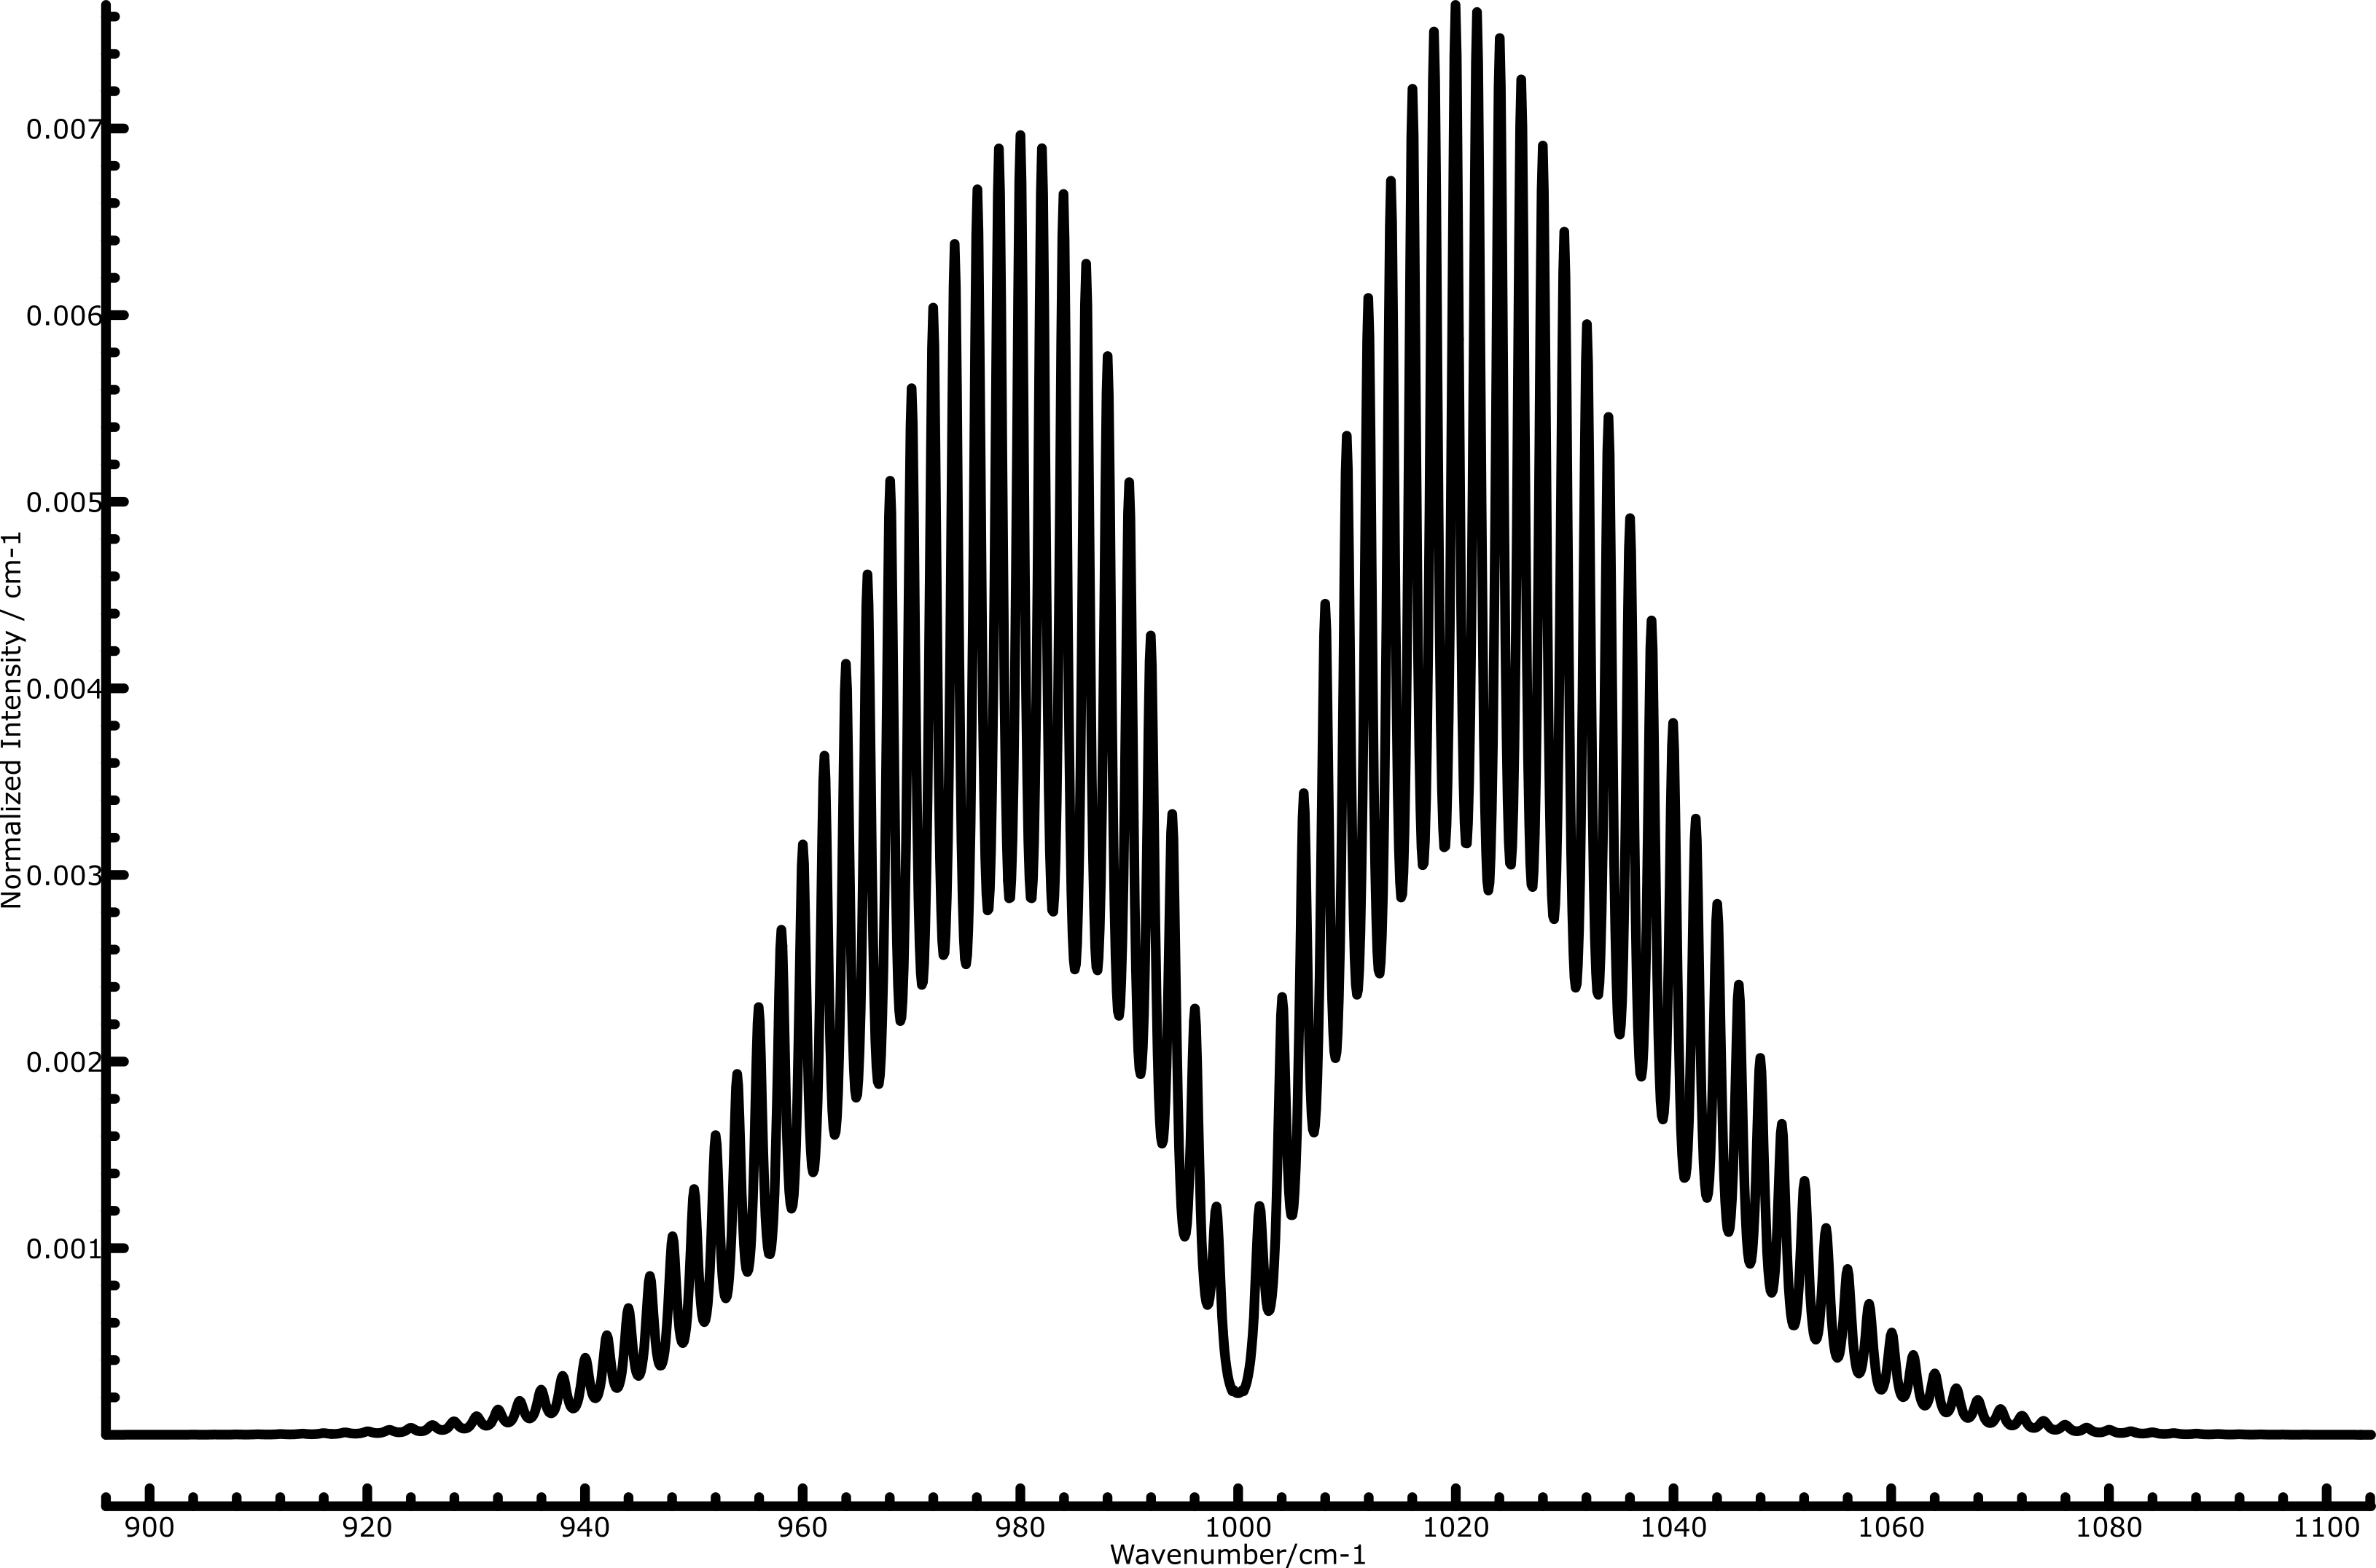
\includegraphics[width=\linewidth]	  					{figures/Lor1.png}
			\end{figure}
				\centering(b) \\
		\end{minipage}
	\end{minipage}
	\captionof{figure}{Linear molecule at 300\si{K} for Gau:1 and Lor:0 (a) and for Gau:0 and Lor:1 (b) }
		\label{fig:lorgau}
\end{center}
If the temperature is increased the spectrum get wider; the range of wavenumbers is increased. The intensity decreases with an increase in temperature. The increase in temperature increases the spread in the rotational quantum number and therefore the intensity is decreased. If the temperature is increased, so is the thermal energy ($k_B T$), and more vibrational states can be excited, hence the broader spectrum. The population of vibrational states
\begin{equation}
	N_v = N_0 \dfrac{\exp \lbrace\sfrac{E_v}{k_B T}\rbrace}{Z_{vib}(T)}
\end{equation}
show that when the temperature is increased, the population states increase as well. Of course for decreasing temperature the effects are reversed.

\subsection{}
In the final part of the assignment the \ce{MgO} spectrum has to be replicated. First the origin is calculated  
\begin{equation}
	E = T_e + \omega_e (\nu + 0.5) + B_{ev} J (J+1)
\end{equation}
using the fact that $J$ is equal to zero and the origin is equal to the energy. $\nu$ can be either 0 or 1, depending on the state, $\omega_e$ is equal to 785.2183. For $T_e$ the value of 3563.8377 \si{\per \cm} for the $A$ state. This results in a incorrect answer since the origin already given is not the same as the origin calculated, so probably something went wrong in either the calculation or in the selection of the values. I'm afraid I'm out of time to do further investigation on how to correct this error, so I'll assume the current origin values, as given in the template. Furthermore, I think the Ground X ($v=0$) is used and the Excited A ($v=1$) is used in combination with  $<v=1|T(1)|v=0>$. The value for $B_A$ is 0.4906403 and for $B_X$ is 0.56289586. The model looks quite similar to the experimental data, however at the left side there is an extra peak. 

\begin{figure}[H]
	\centering 
	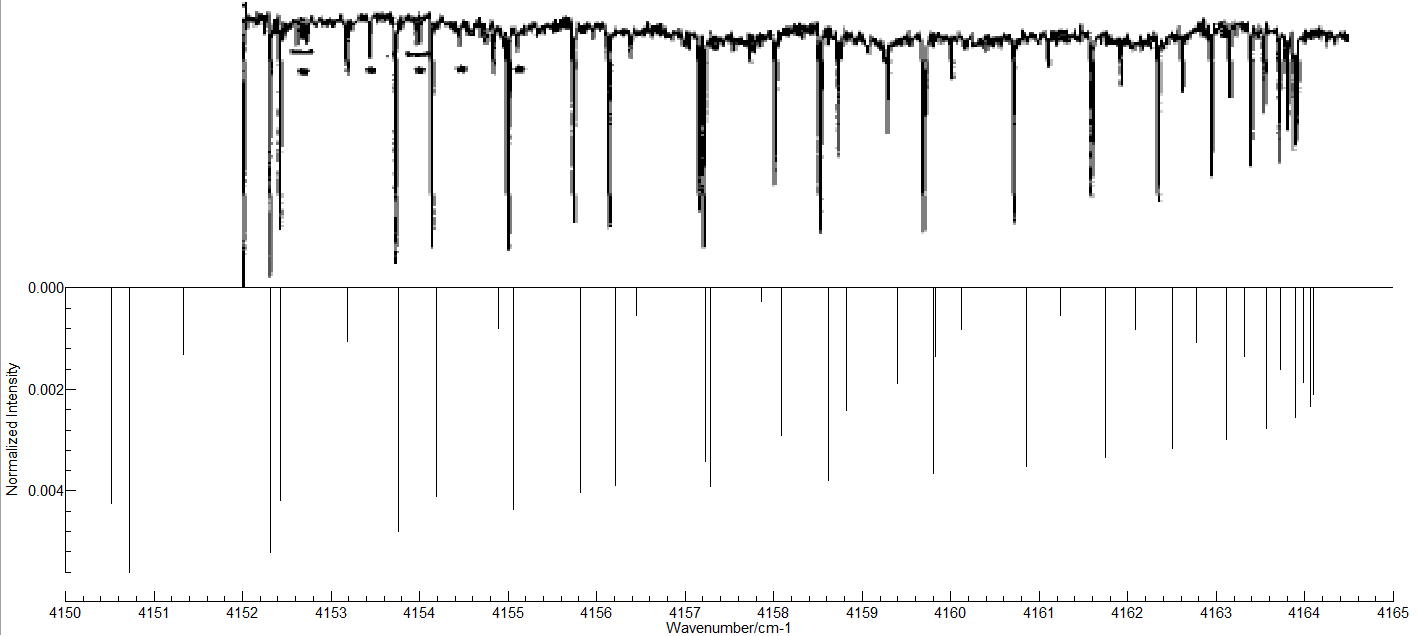
\includegraphics[width=\linewidth]{figures/samen.png}
	\caption{Comparison between model and experimental \ce{MgO} spectrum}
\end{figure} 

\newpage                           
\appendix
\setcounter{section}{1}
\setcounter{subsection}{0}

\subsection{Figures from \ref{ch3}} \label{Appendix}
\begin{center}
	\begin{minipage}{\linewidth}
		\begin{minipage}{0.5\linewidth}
			\begin{figure}[H]
				\centering 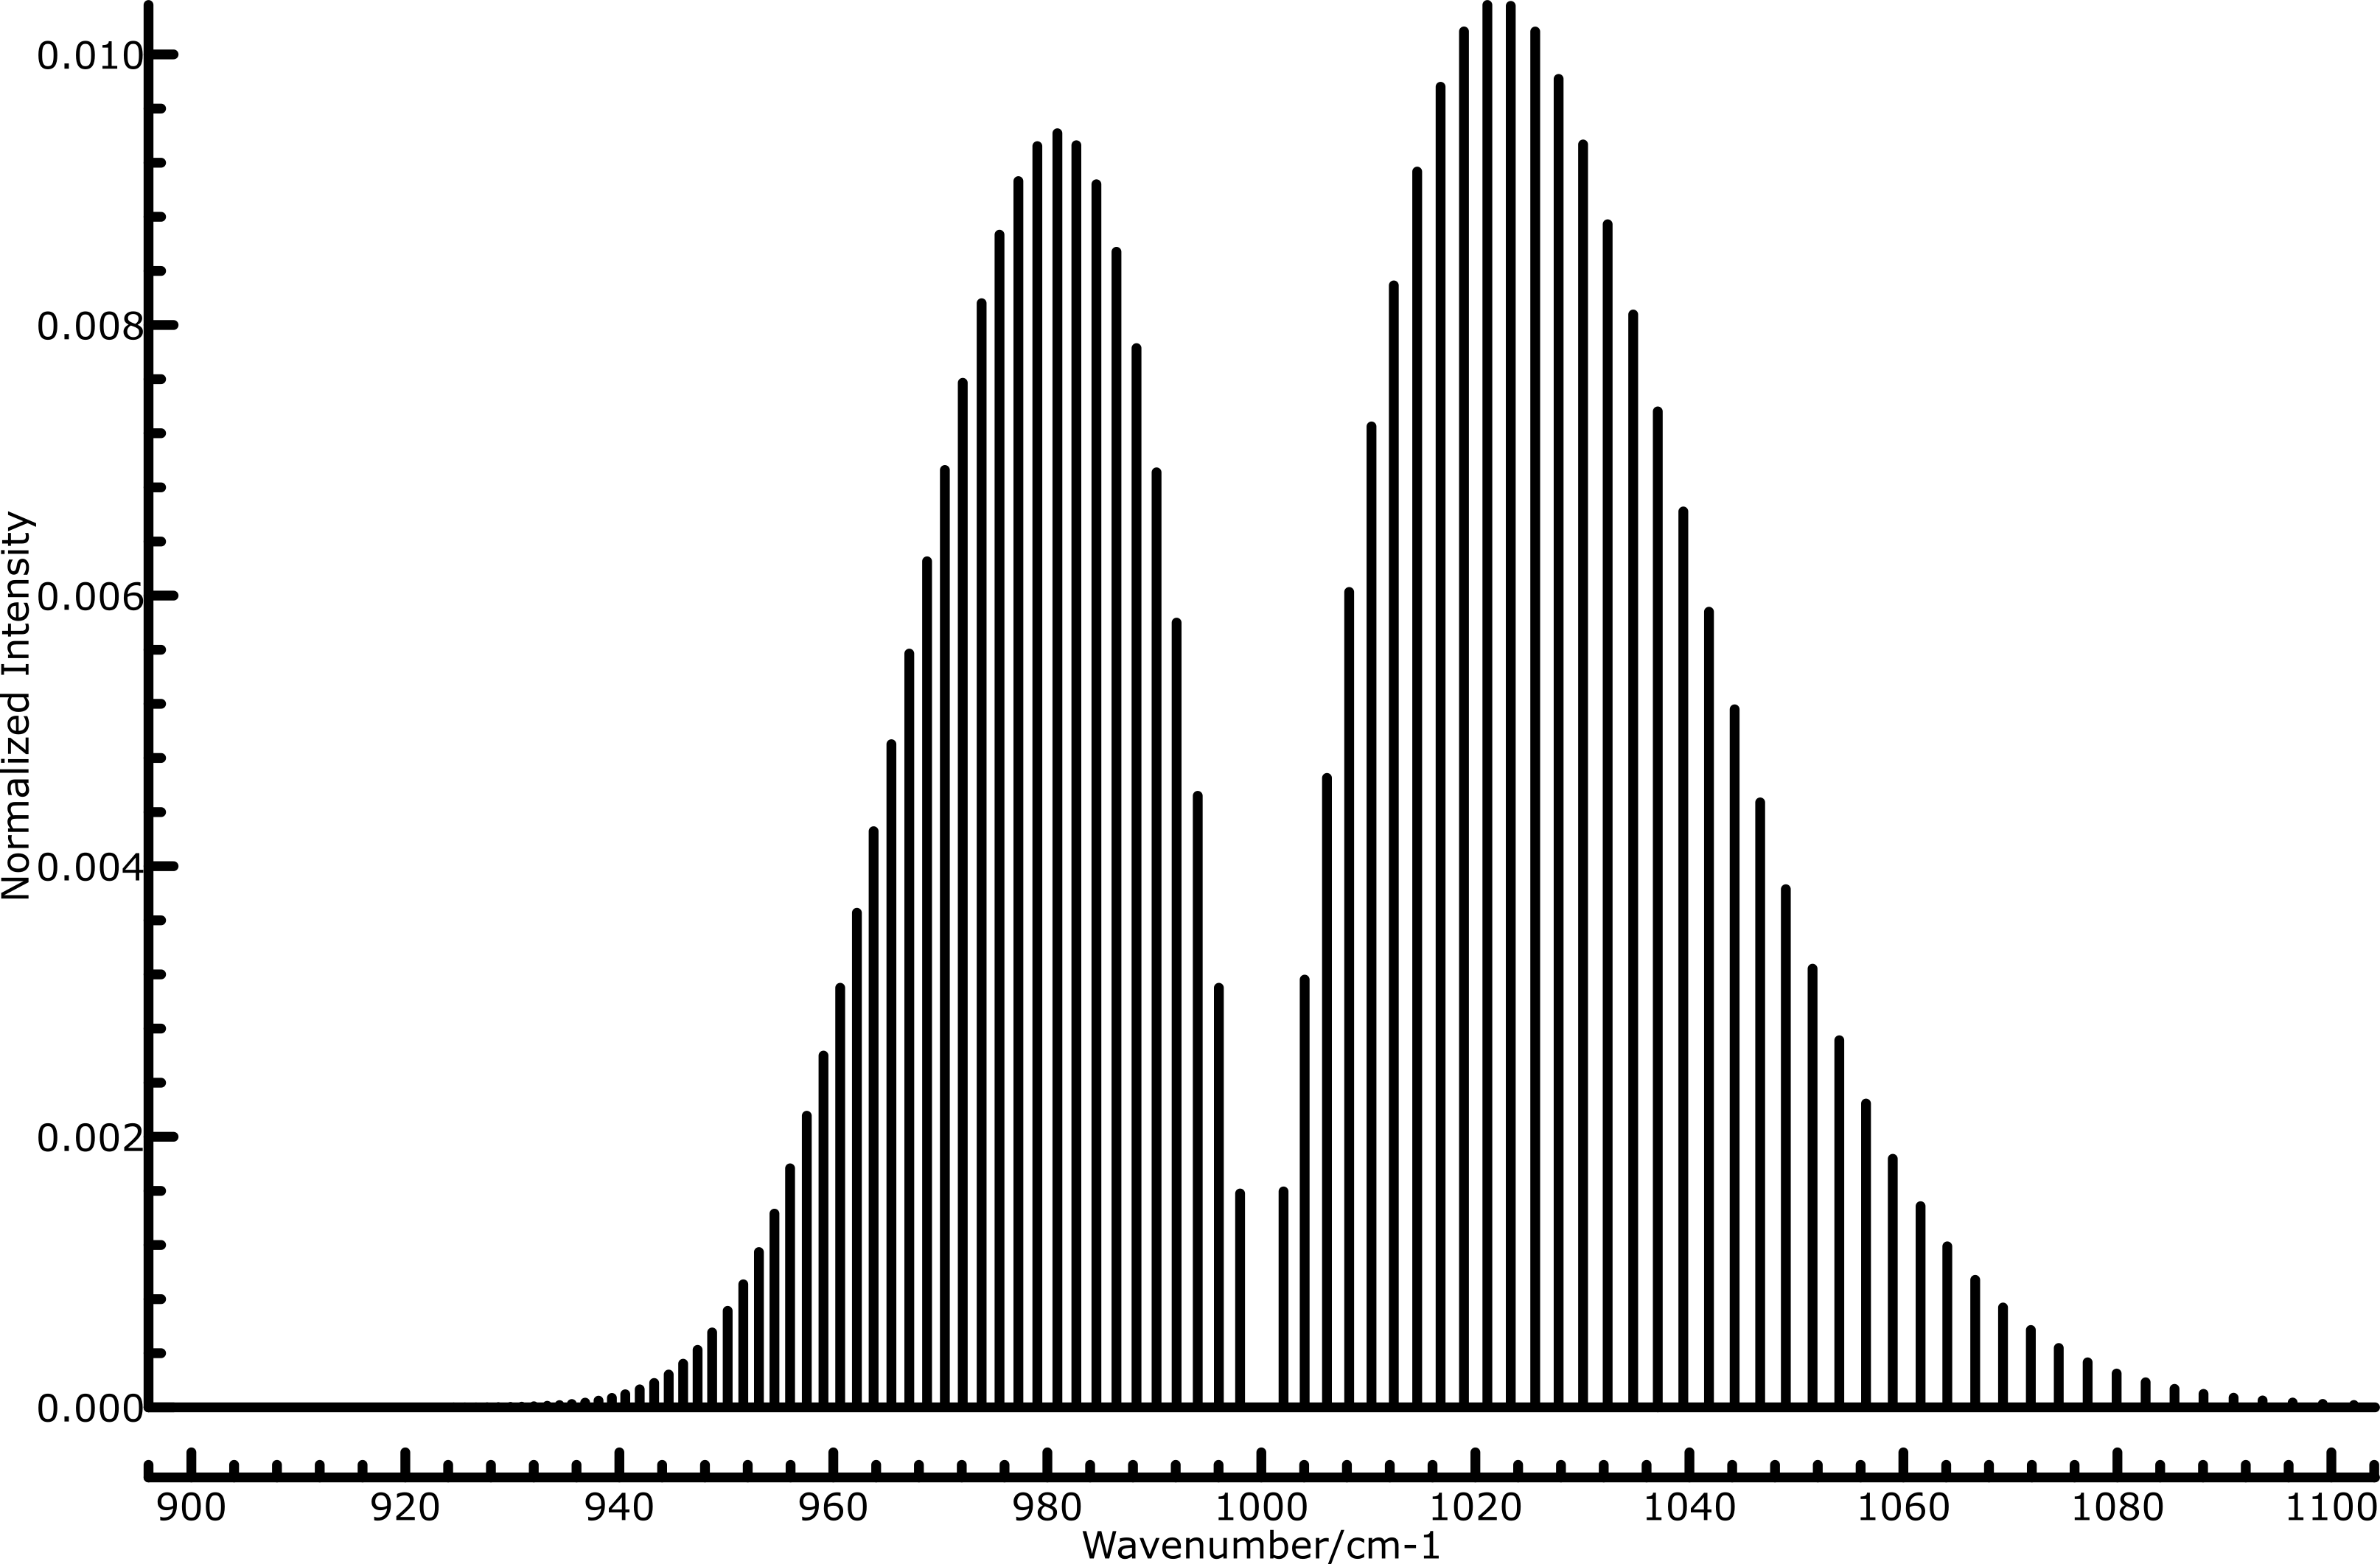
\includegraphics[width=\linewidth] 						{figures/B101.png}
			\end{figure} 
				\centering(B = 1.01) \\
		\end{minipage}
		\begin{minipage}{0.5\linewidth}
		   \begin{figure}[H]
				\centering 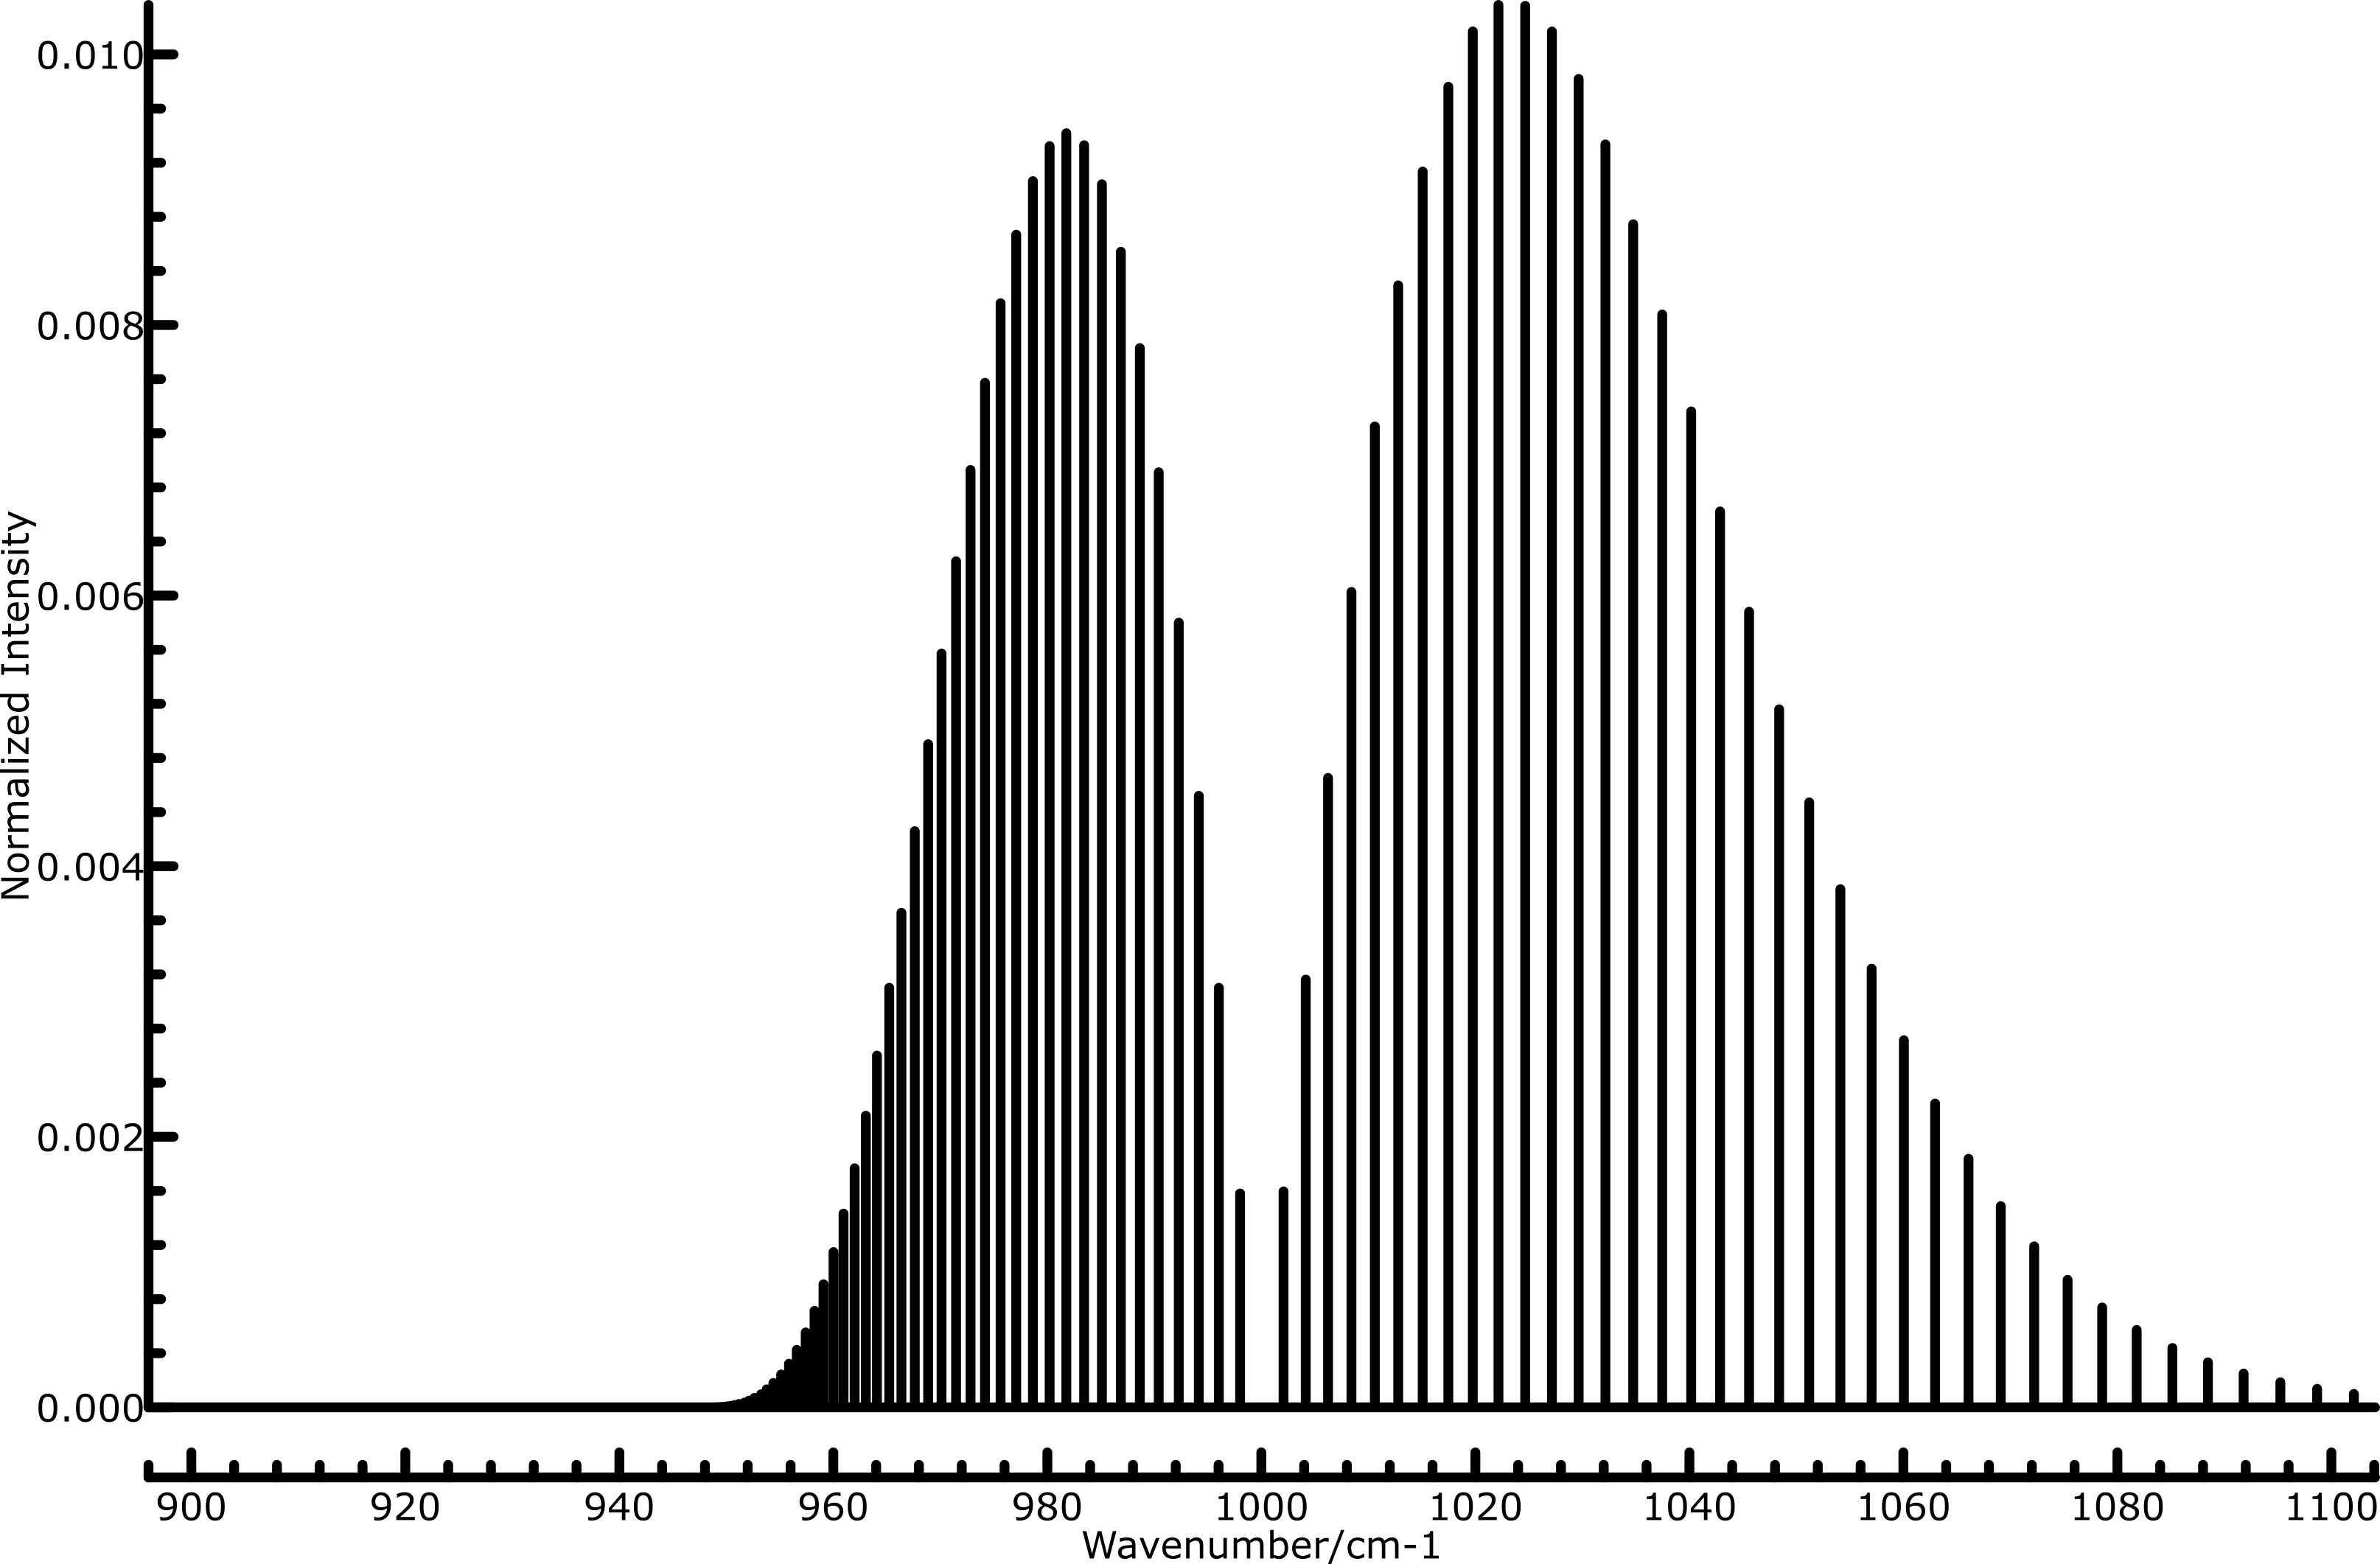
\includegraphics[width=\linewidth]	  					{figures/B102.png}
			\end{figure}
				\centering(B = 1.02) \\
		\end{minipage}
	\end{minipage}
\end{center}
\begin{center}
	\begin{minipage}{\linewidth}
		\begin{minipage}{0.5\linewidth}
			\begin{figure}[H]
				\centering 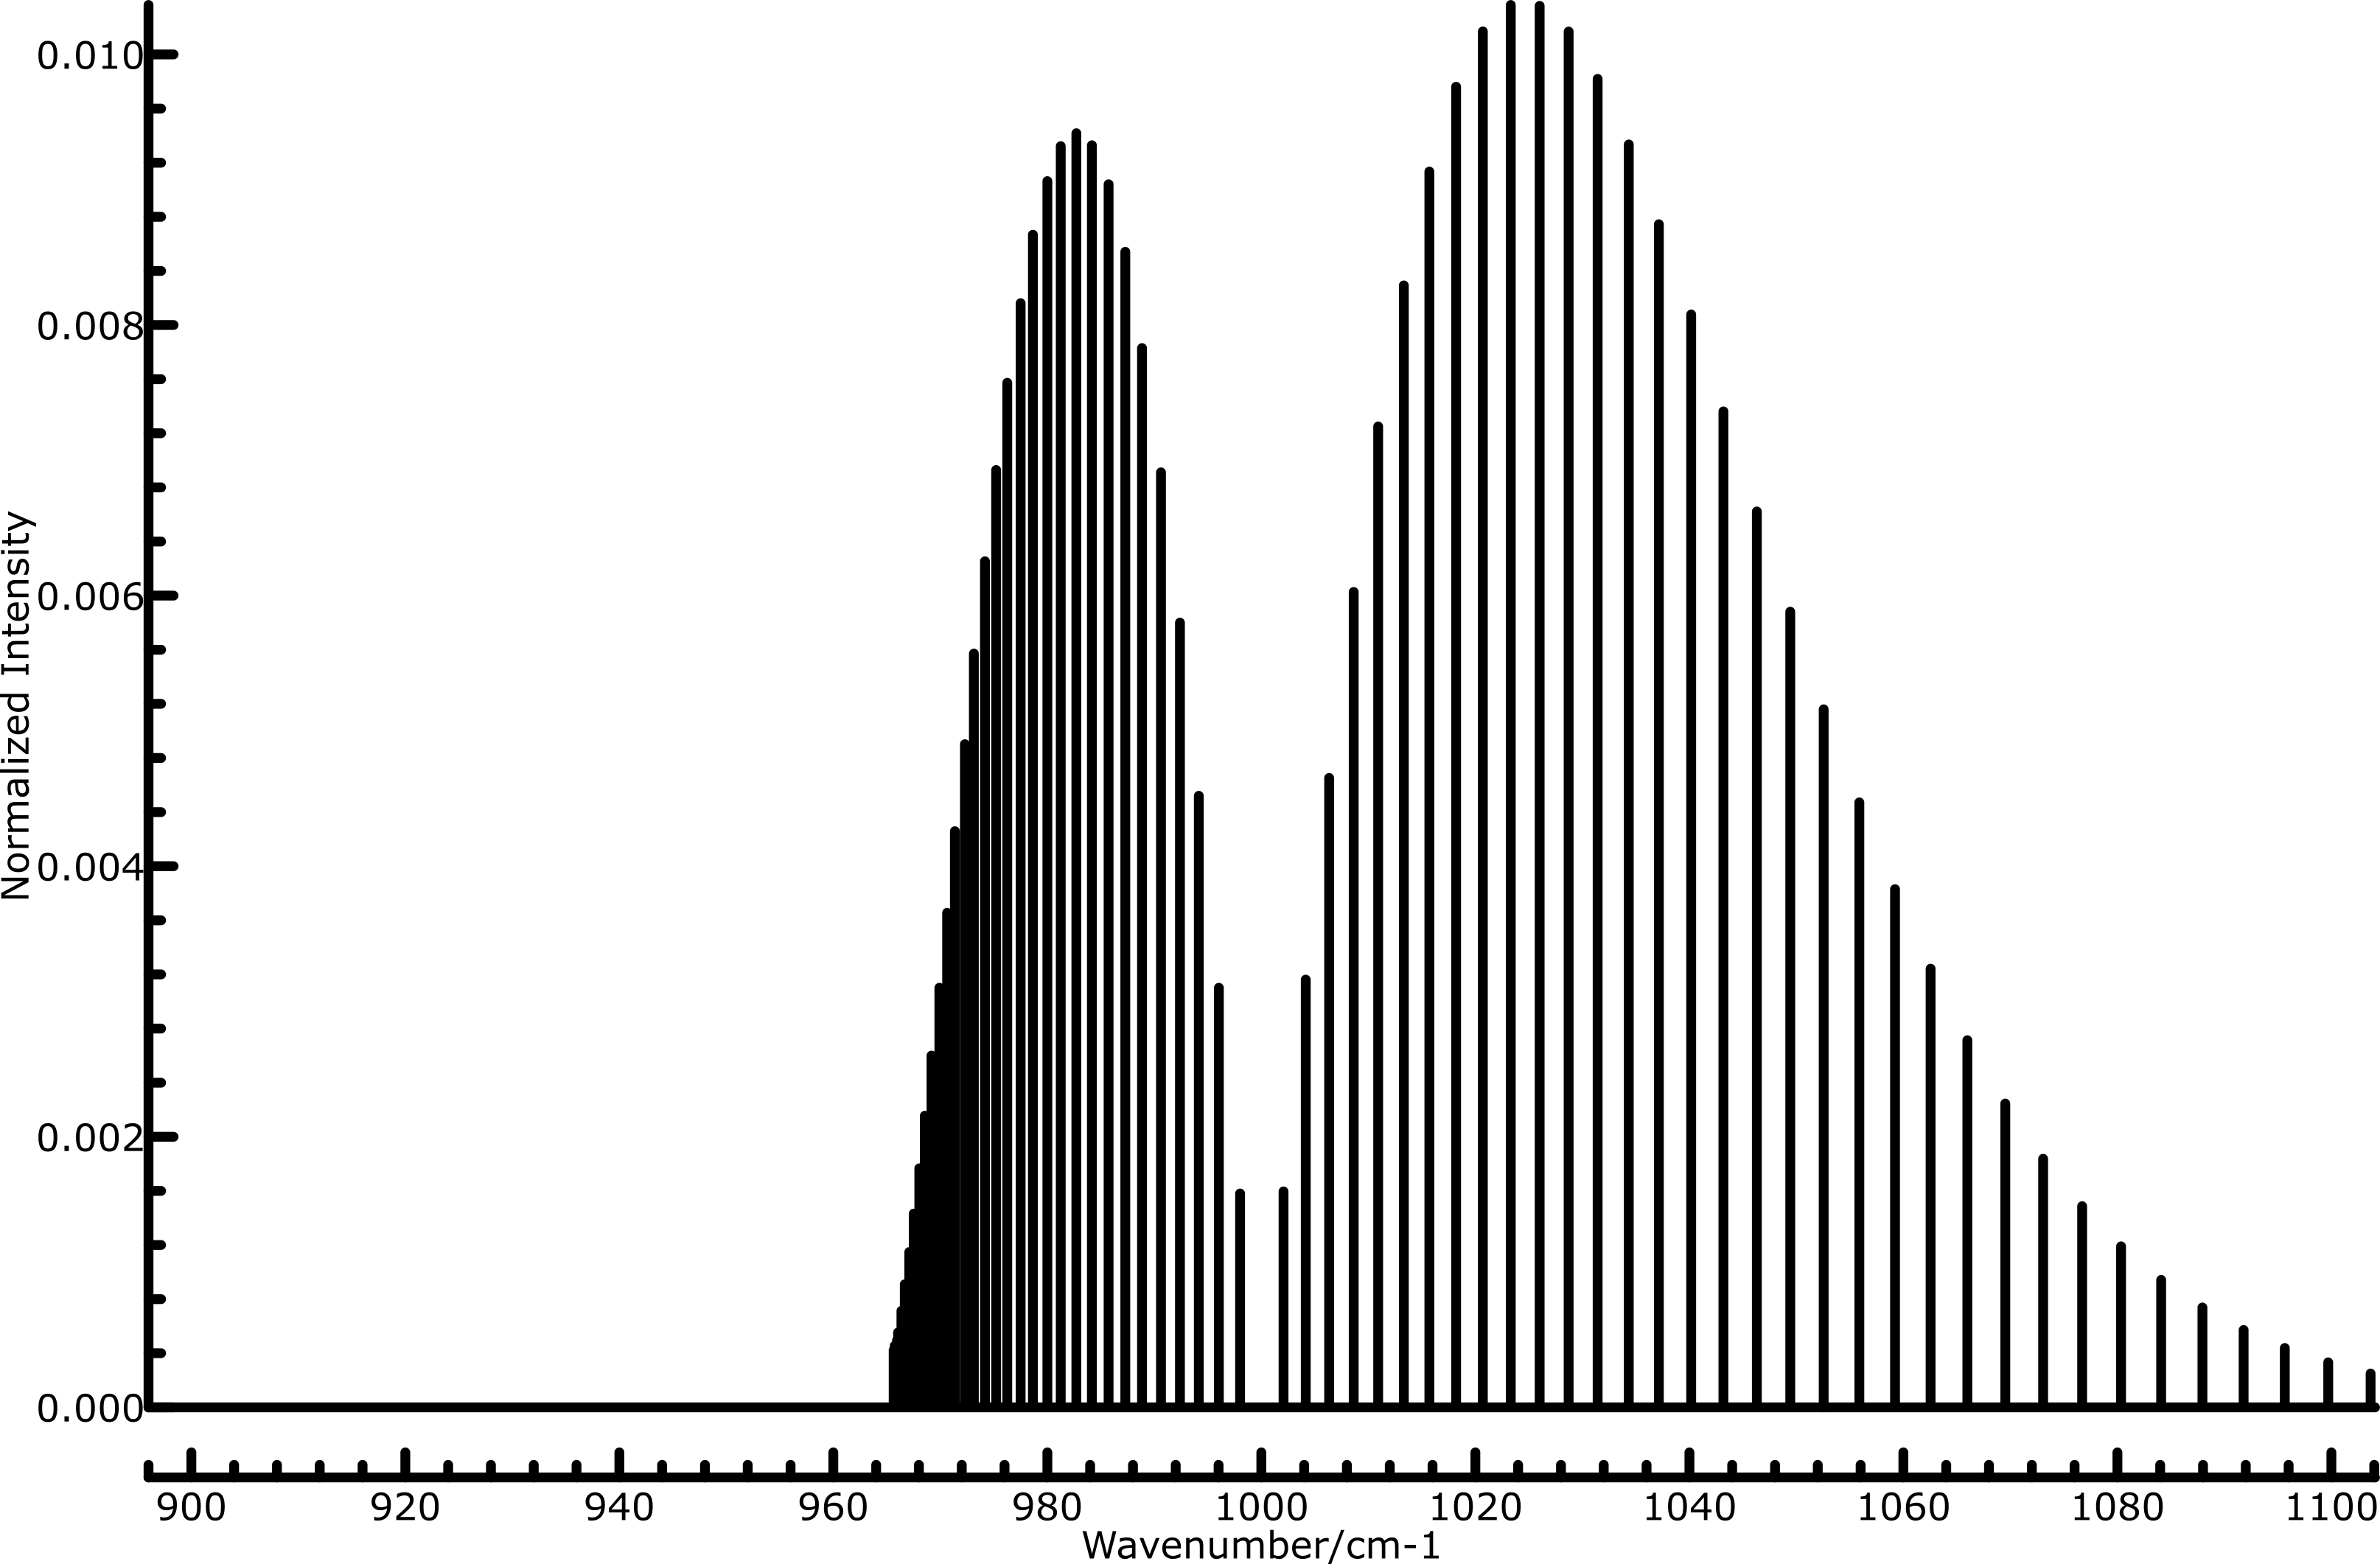
\includegraphics[width=\linewidth] 						{figures/B103.png}
			\end{figure} 
				\centering(B = 1.03) \\
		\end{minipage}
		\begin{minipage}{0.5\linewidth}
		   \begin{figure}[H]
				\centering 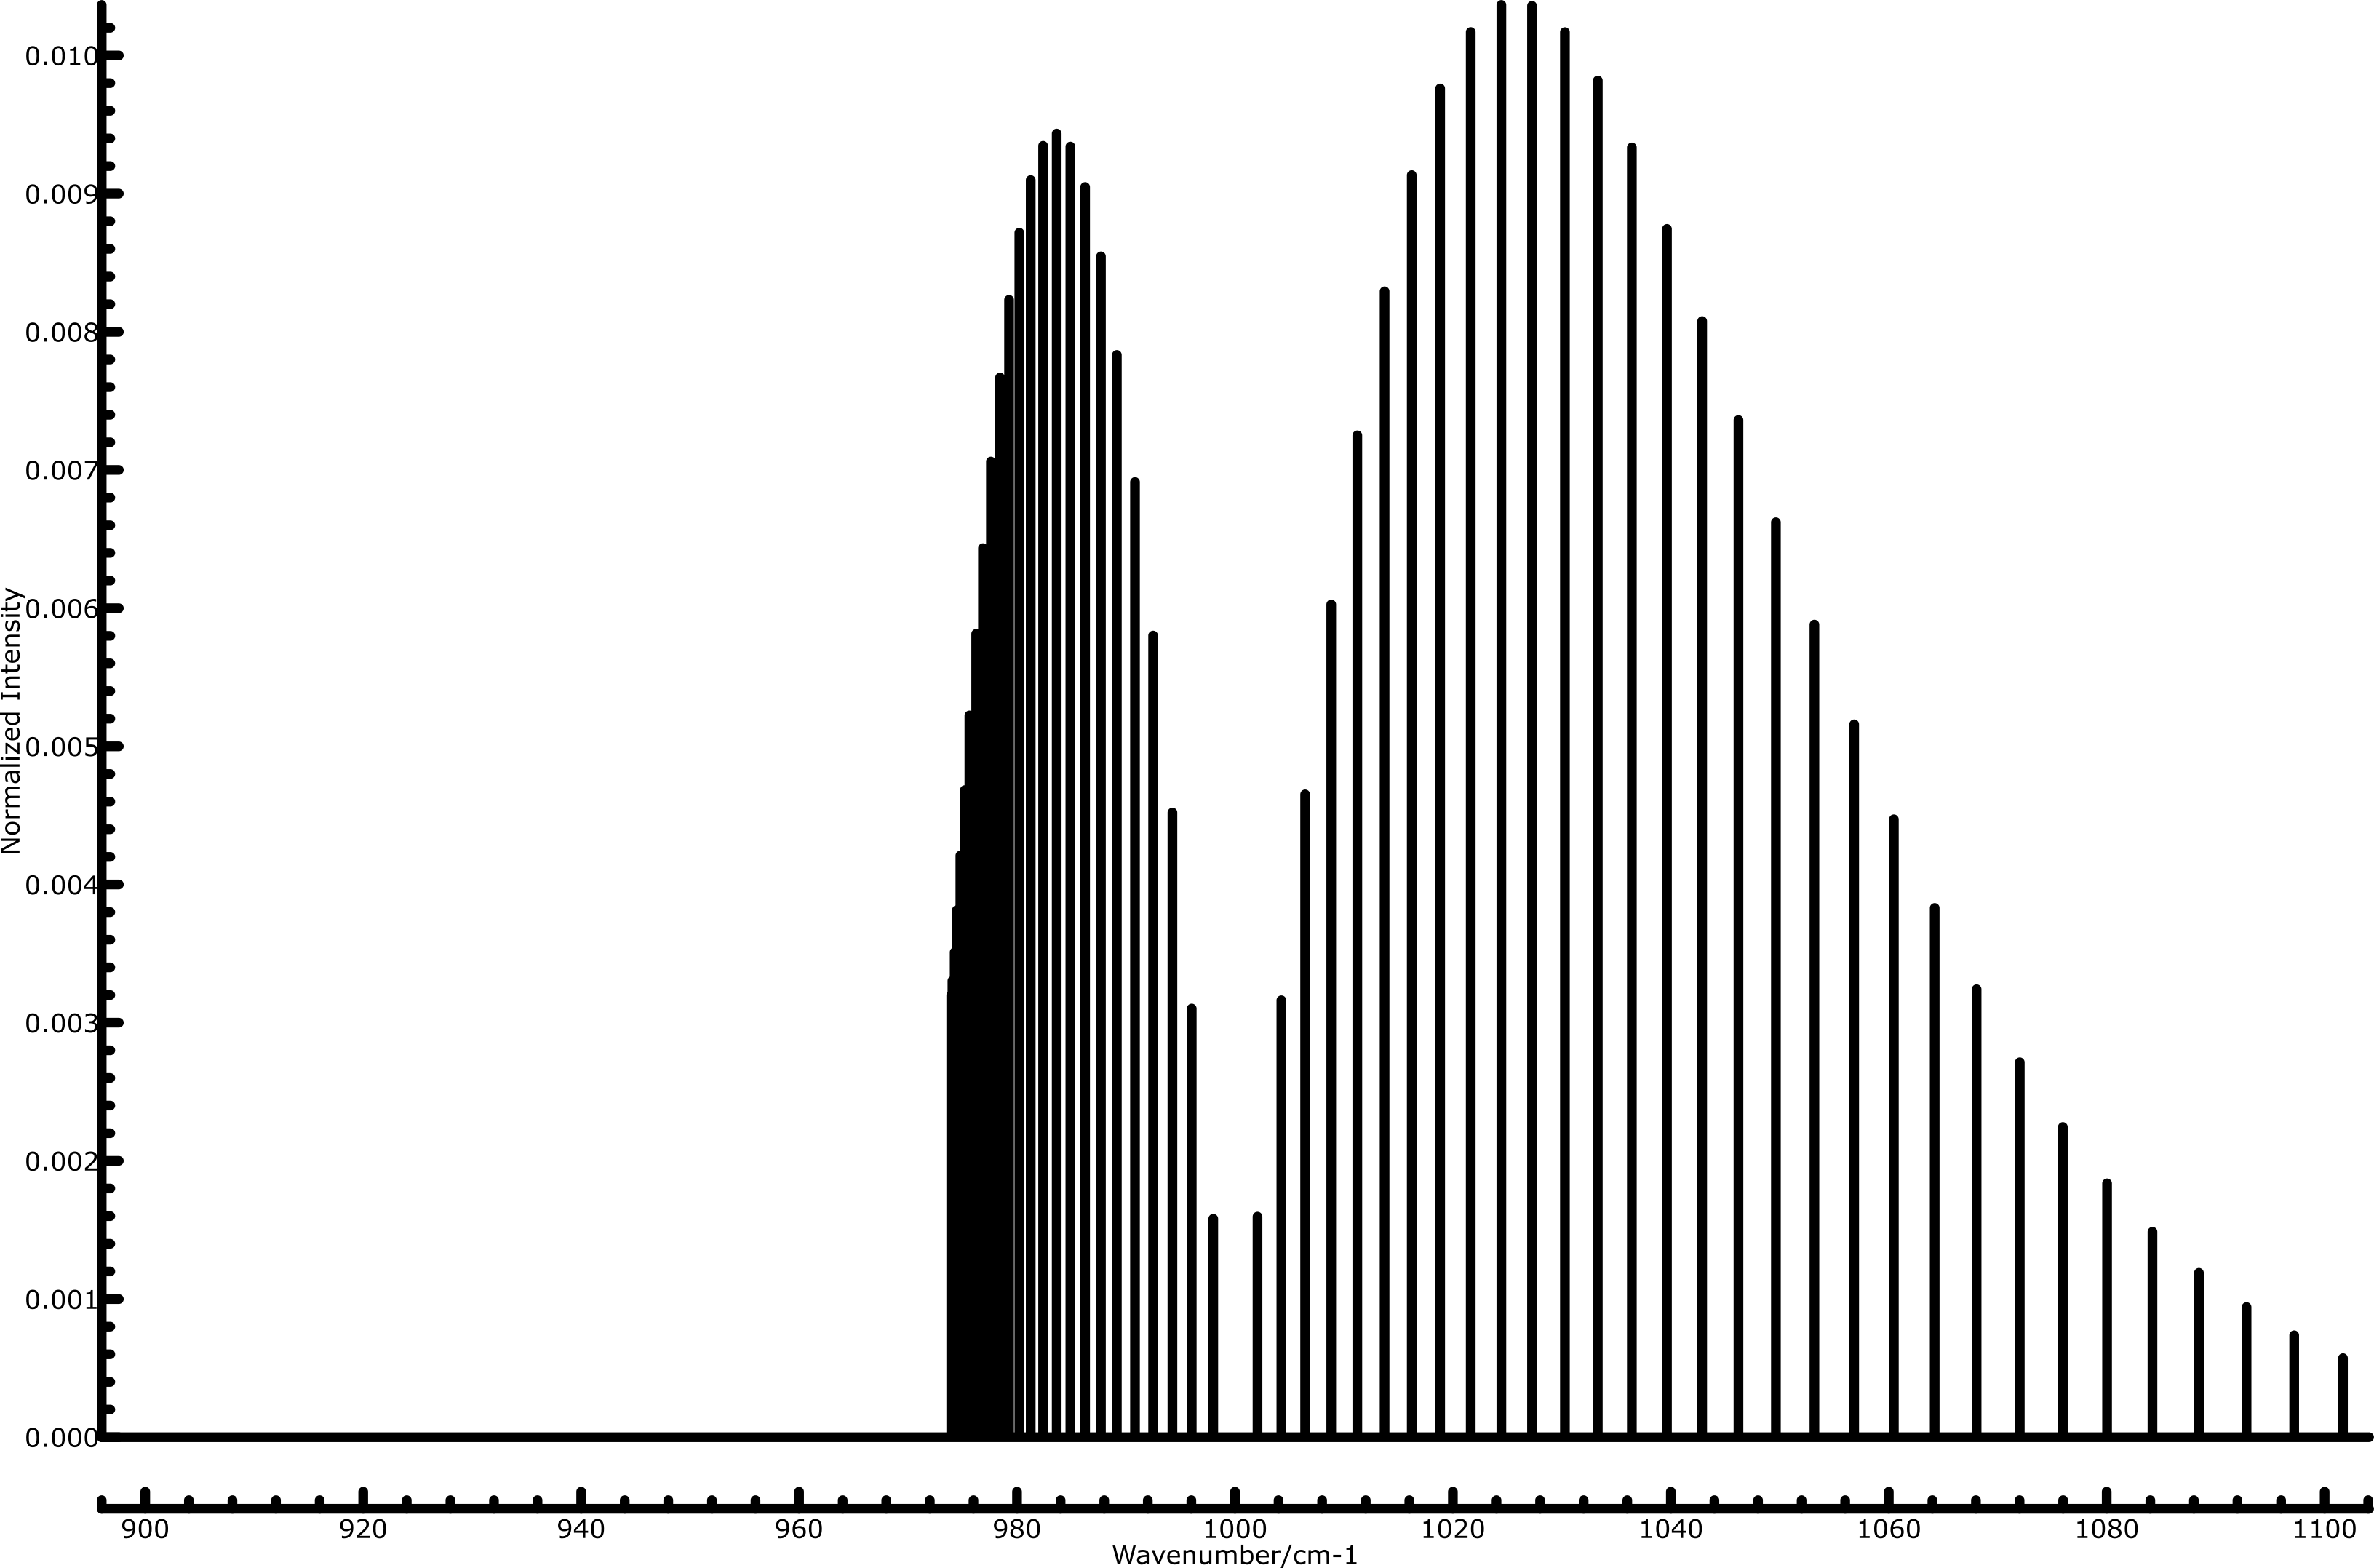
\includegraphics[width=\linewidth]	  					{figures/B104.png}
			\end{figure}
				\centering(B = 1.04) \\
		\end{minipage}
	\end{minipage}
\end{center}
\begin{center}
	\begin{minipage}{\linewidth}
		\begin{minipage}{0.5\linewidth}
			\begin{figure}[H]
				\centering 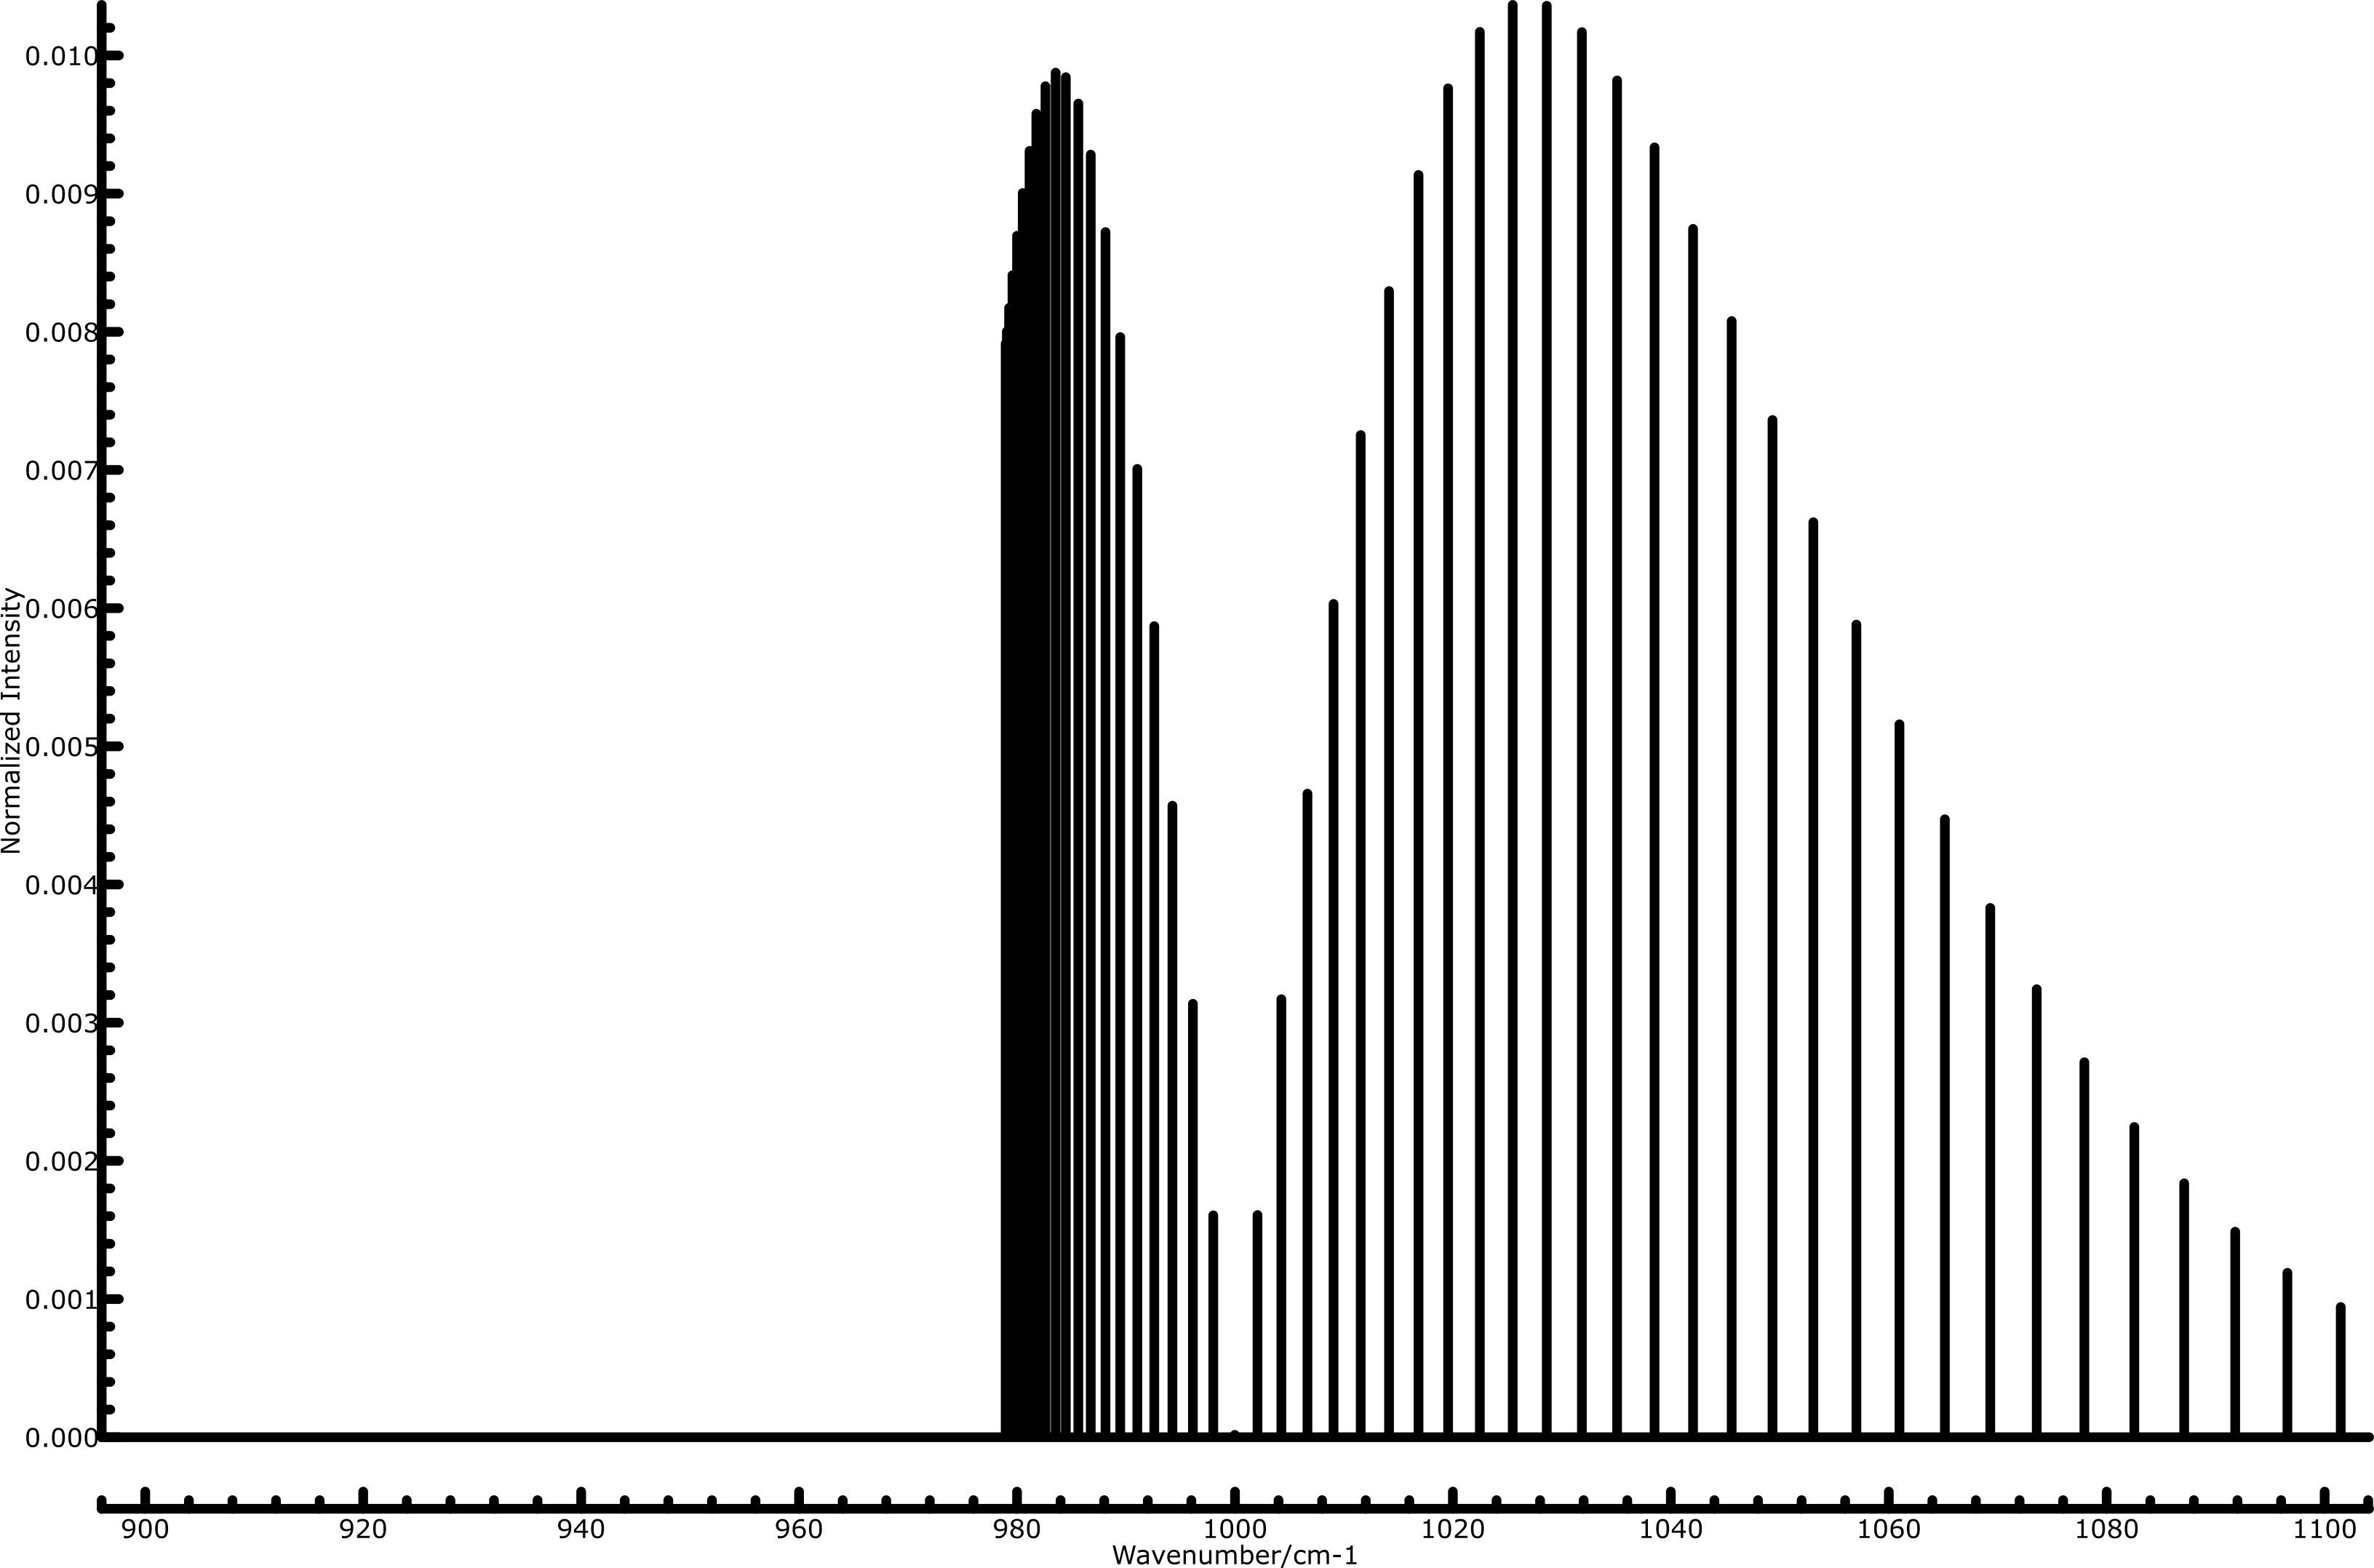
\includegraphics[width=\linewidth] 						{figures/B105.png}
			\end{figure} 
				\centering(B = 1.05) \\
		\end{minipage}
		\begin{minipage}{0.5\linewidth}
		   \begin{figure}[H]
				\centering 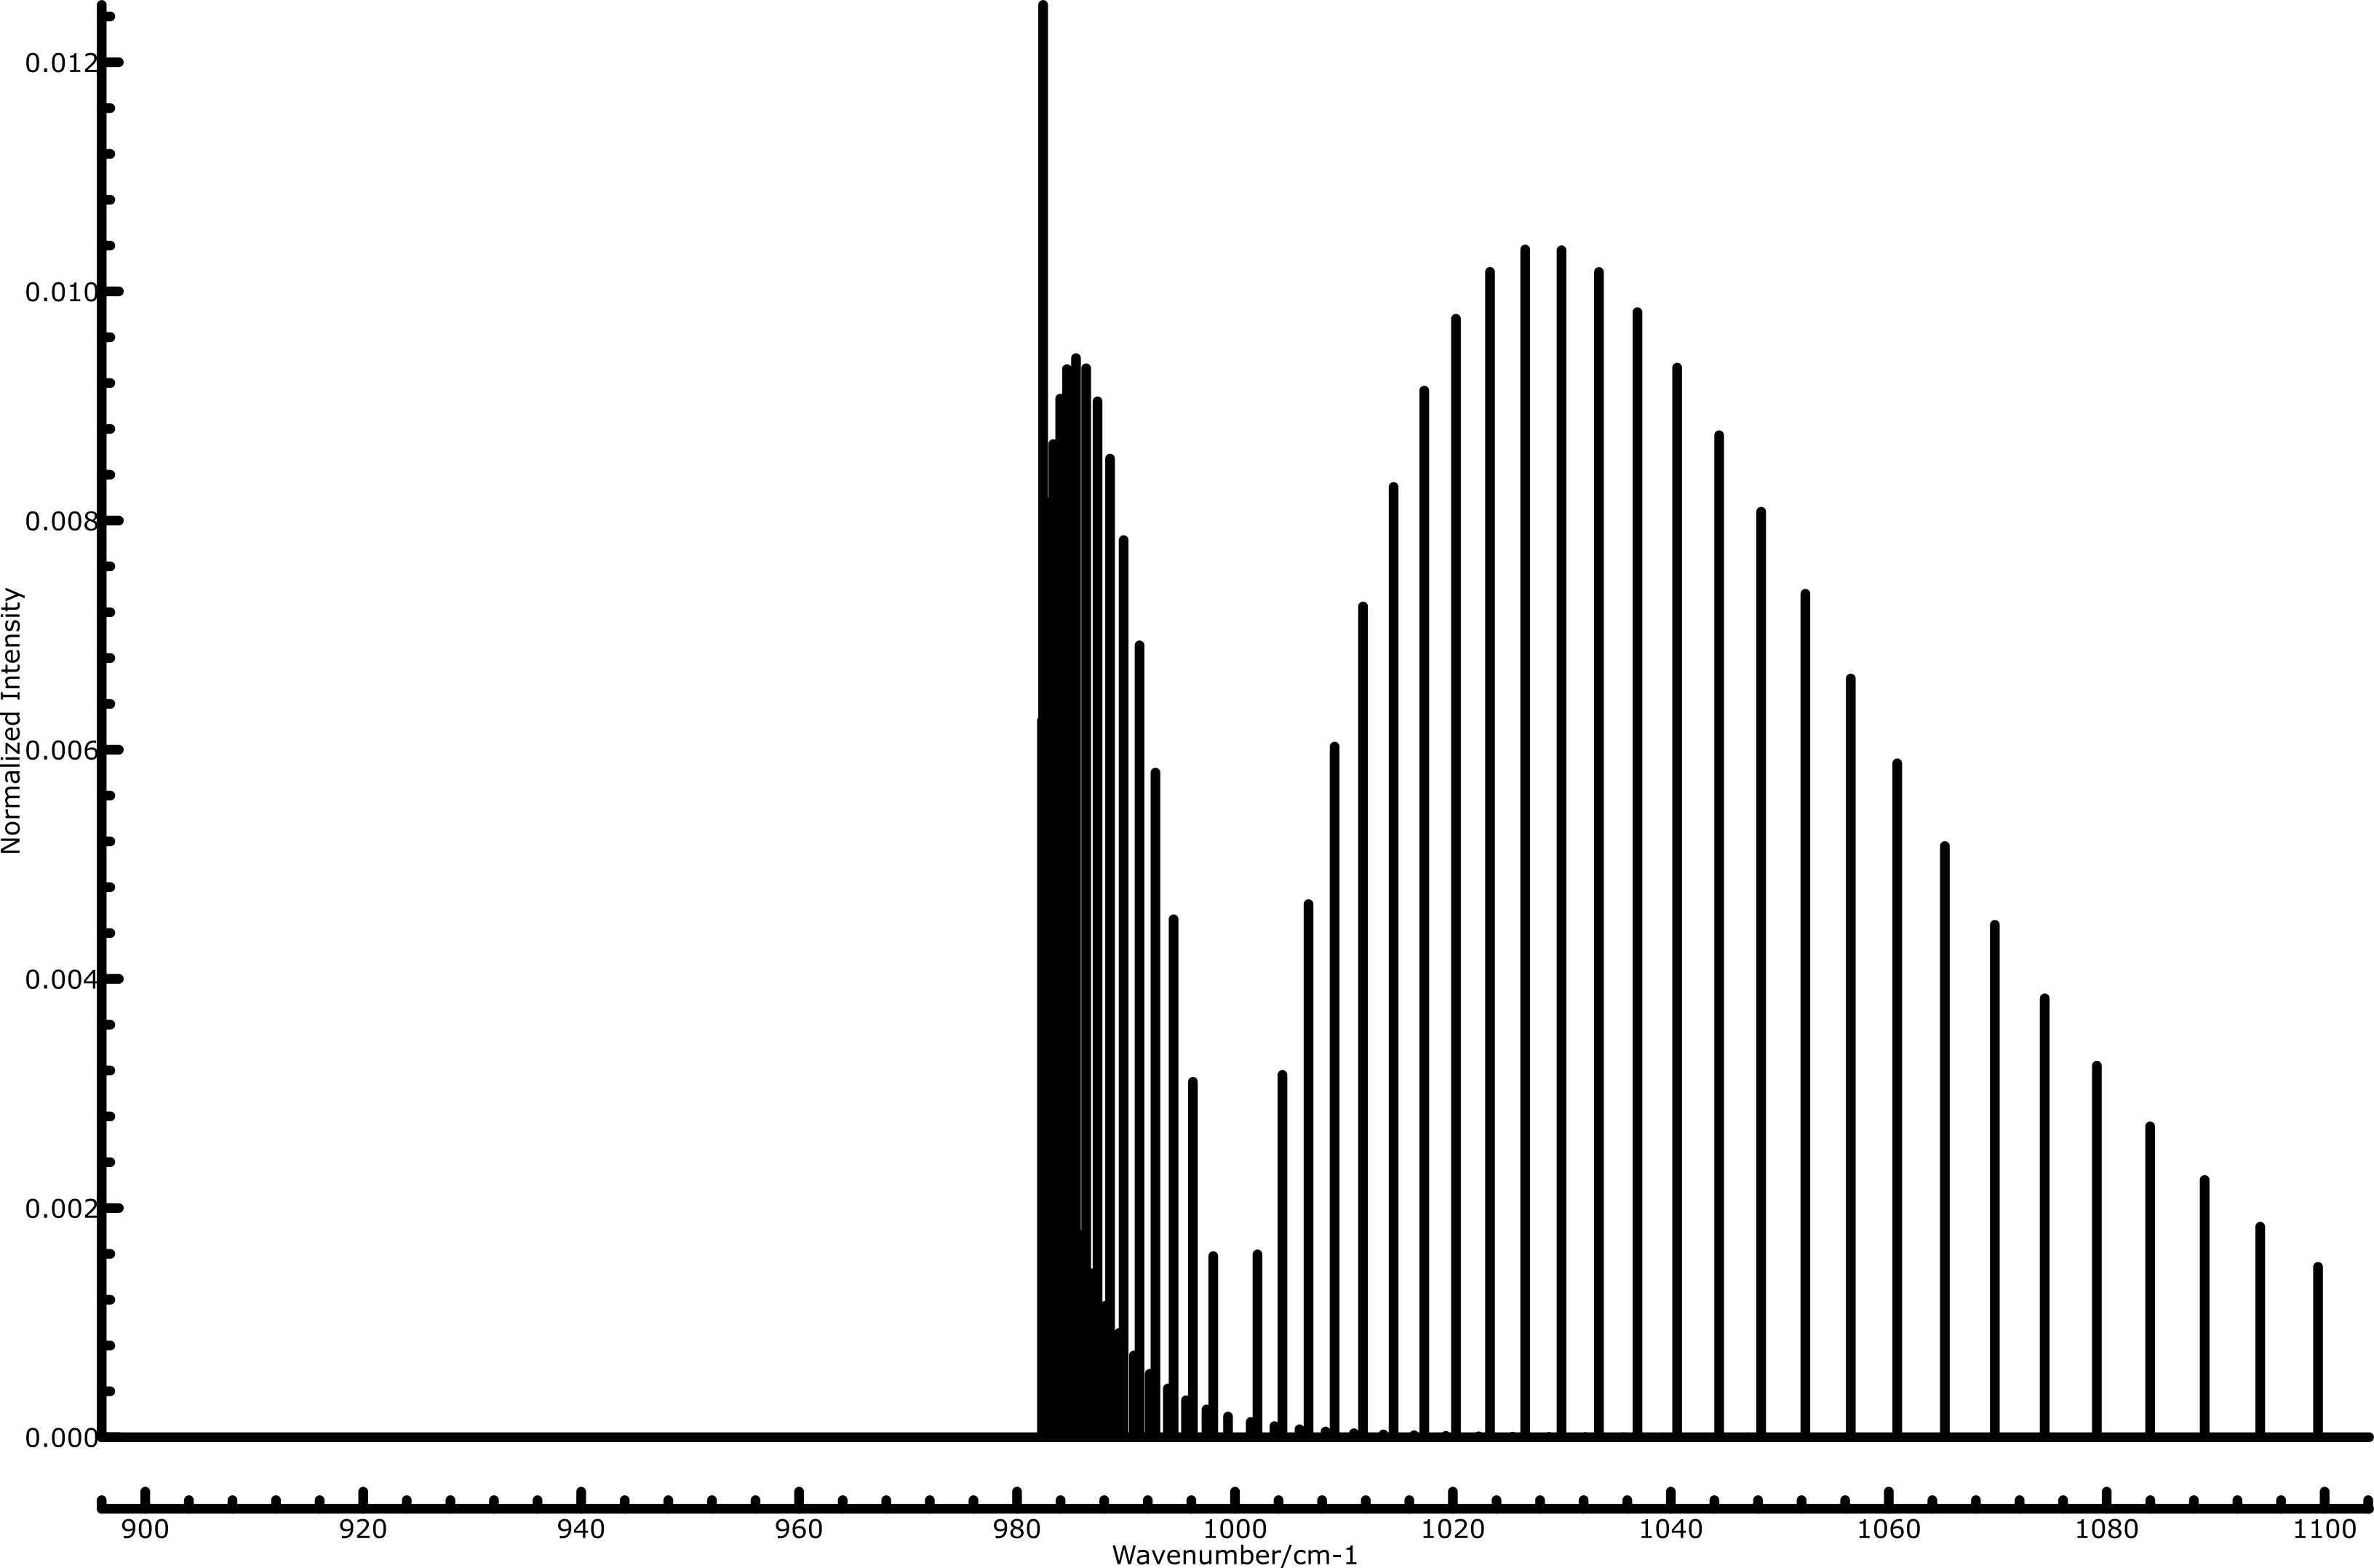
\includegraphics[width=\linewidth]	  					{figures/B106.png}
			\end{figure}
				\centering(B = 1.06) \\
		\end{minipage}
	\end{minipage}
\end{center}
\begin{center}
	\begin{minipage}{\linewidth}
		\begin{minipage}{0.5\linewidth}
			\begin{figure}[H]
				\centering 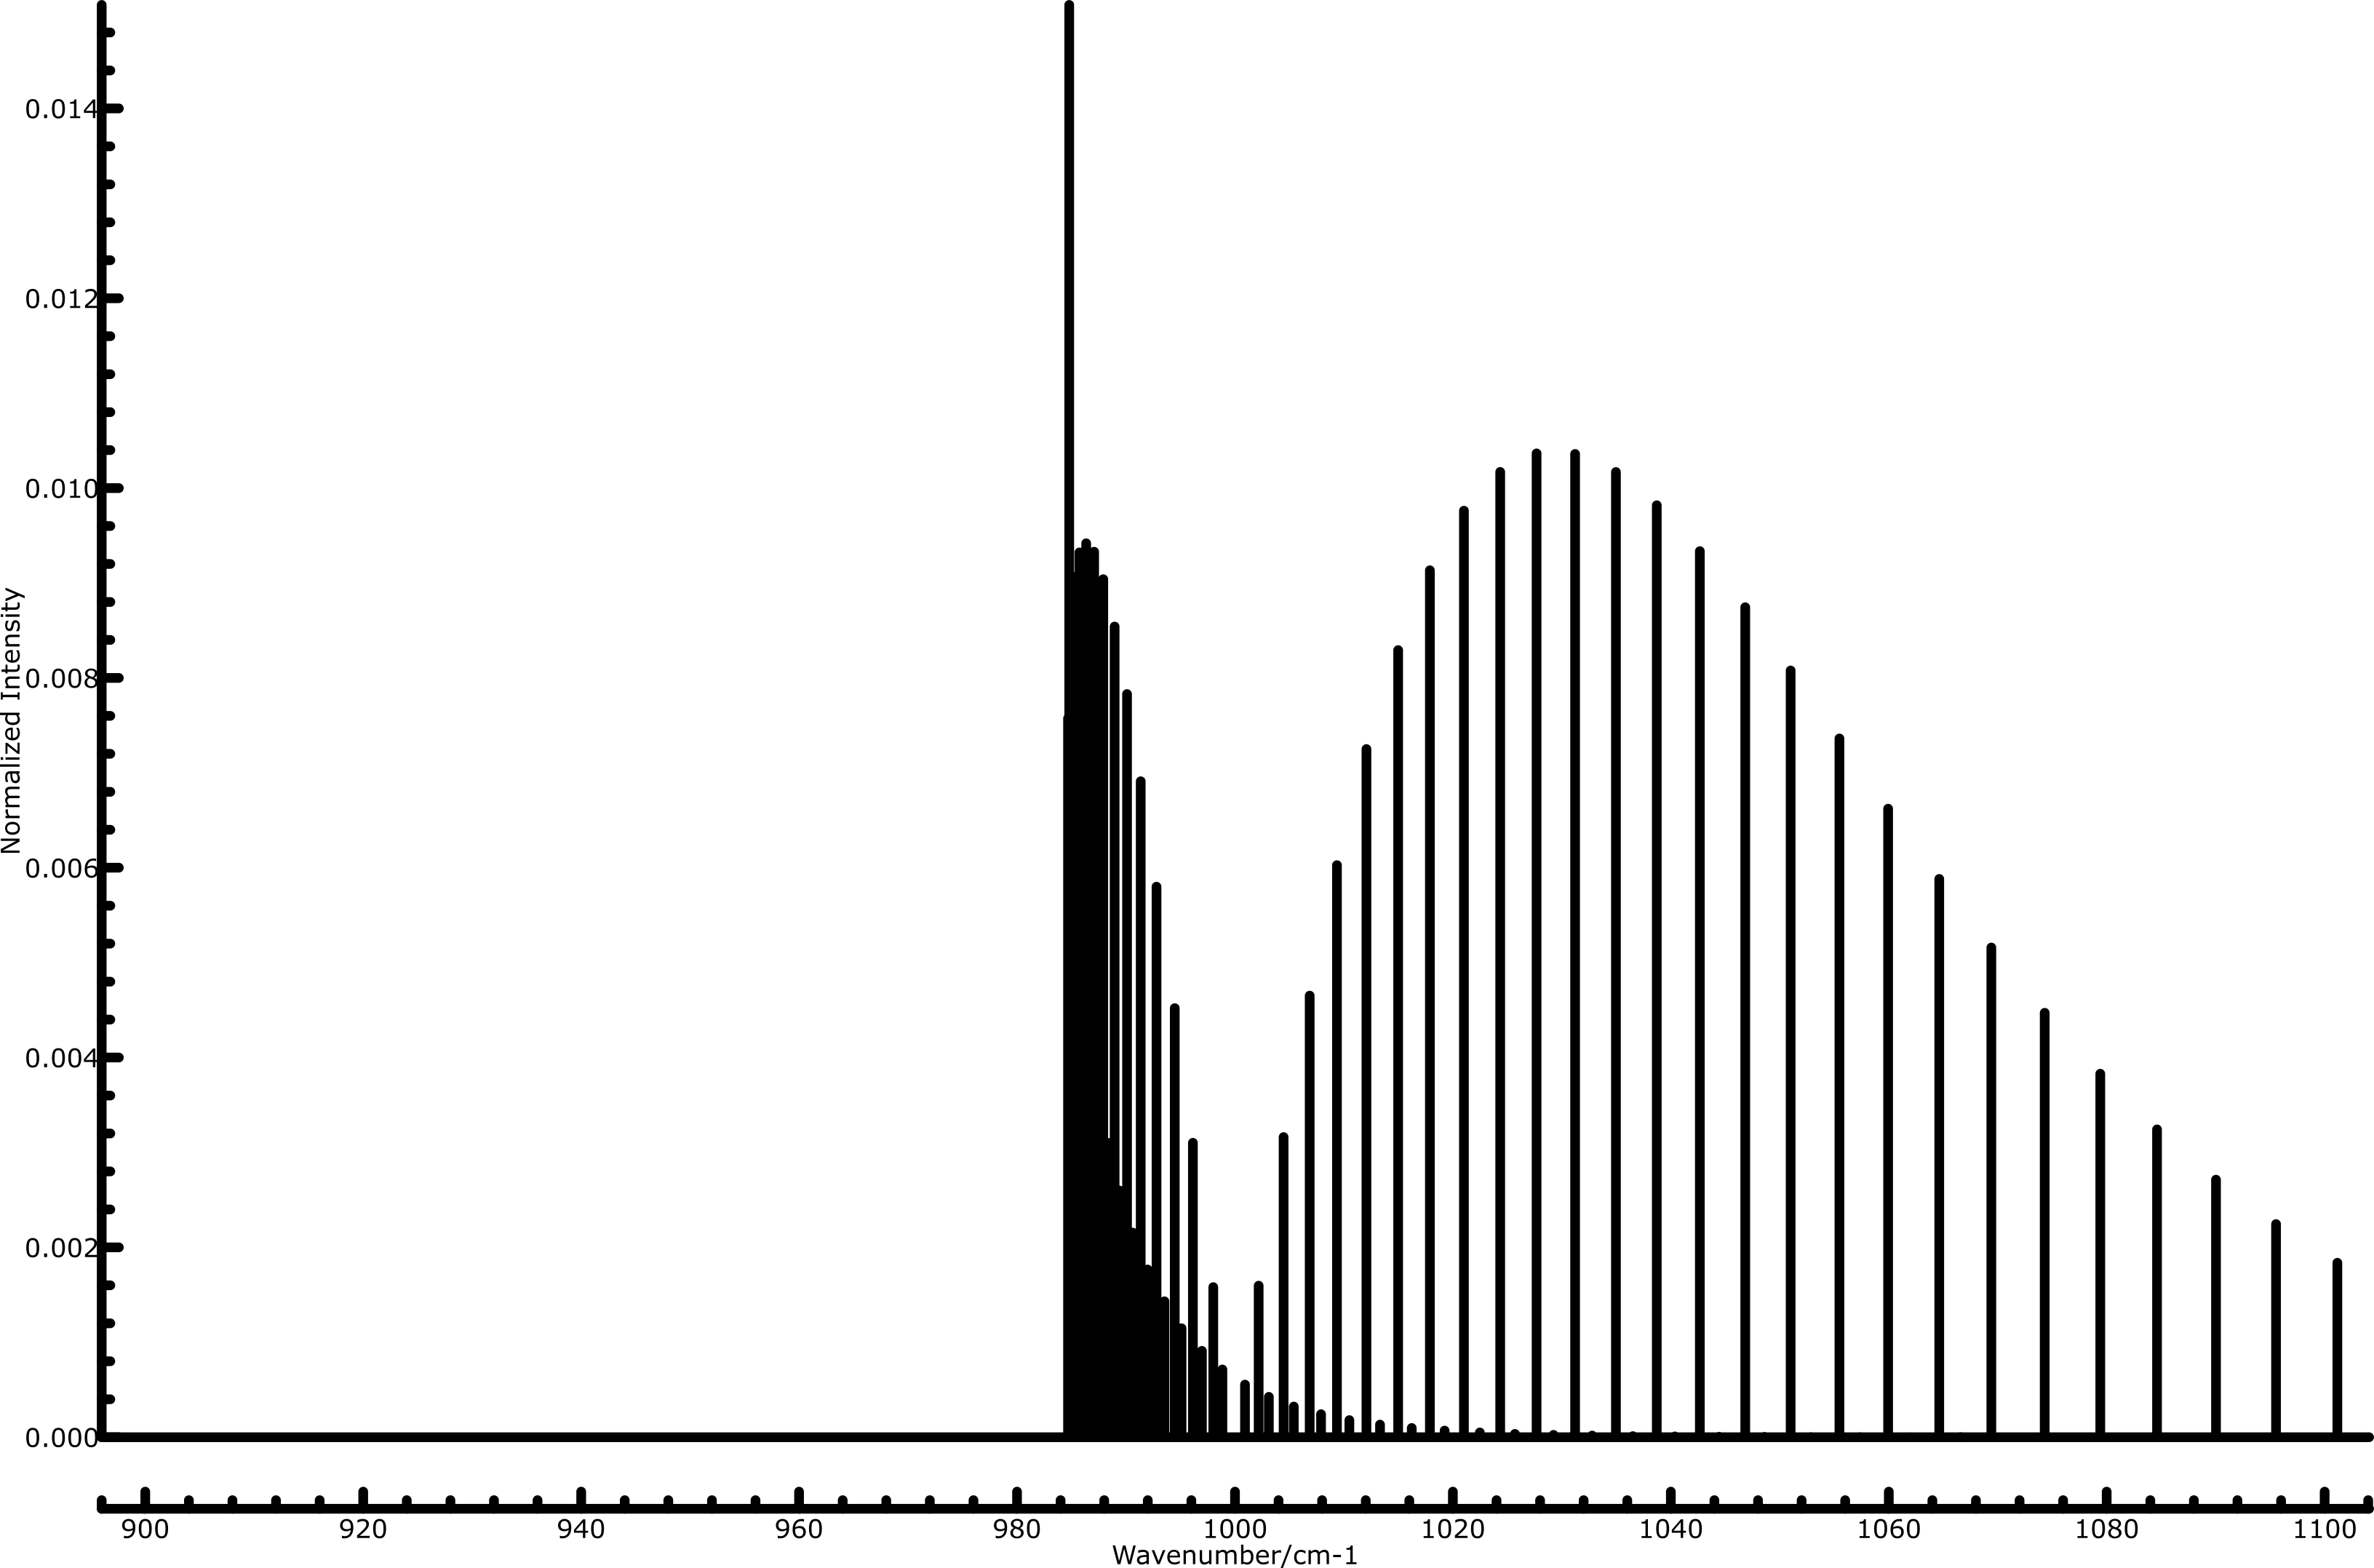
\includegraphics[width=\linewidth] 						{figures/B107.png}
			\end{figure} 
				\centering(B = 1.07) \\
		\end{minipage}
		\begin{minipage}{0.5\linewidth}
		   \begin{figure}[H]
				\centering 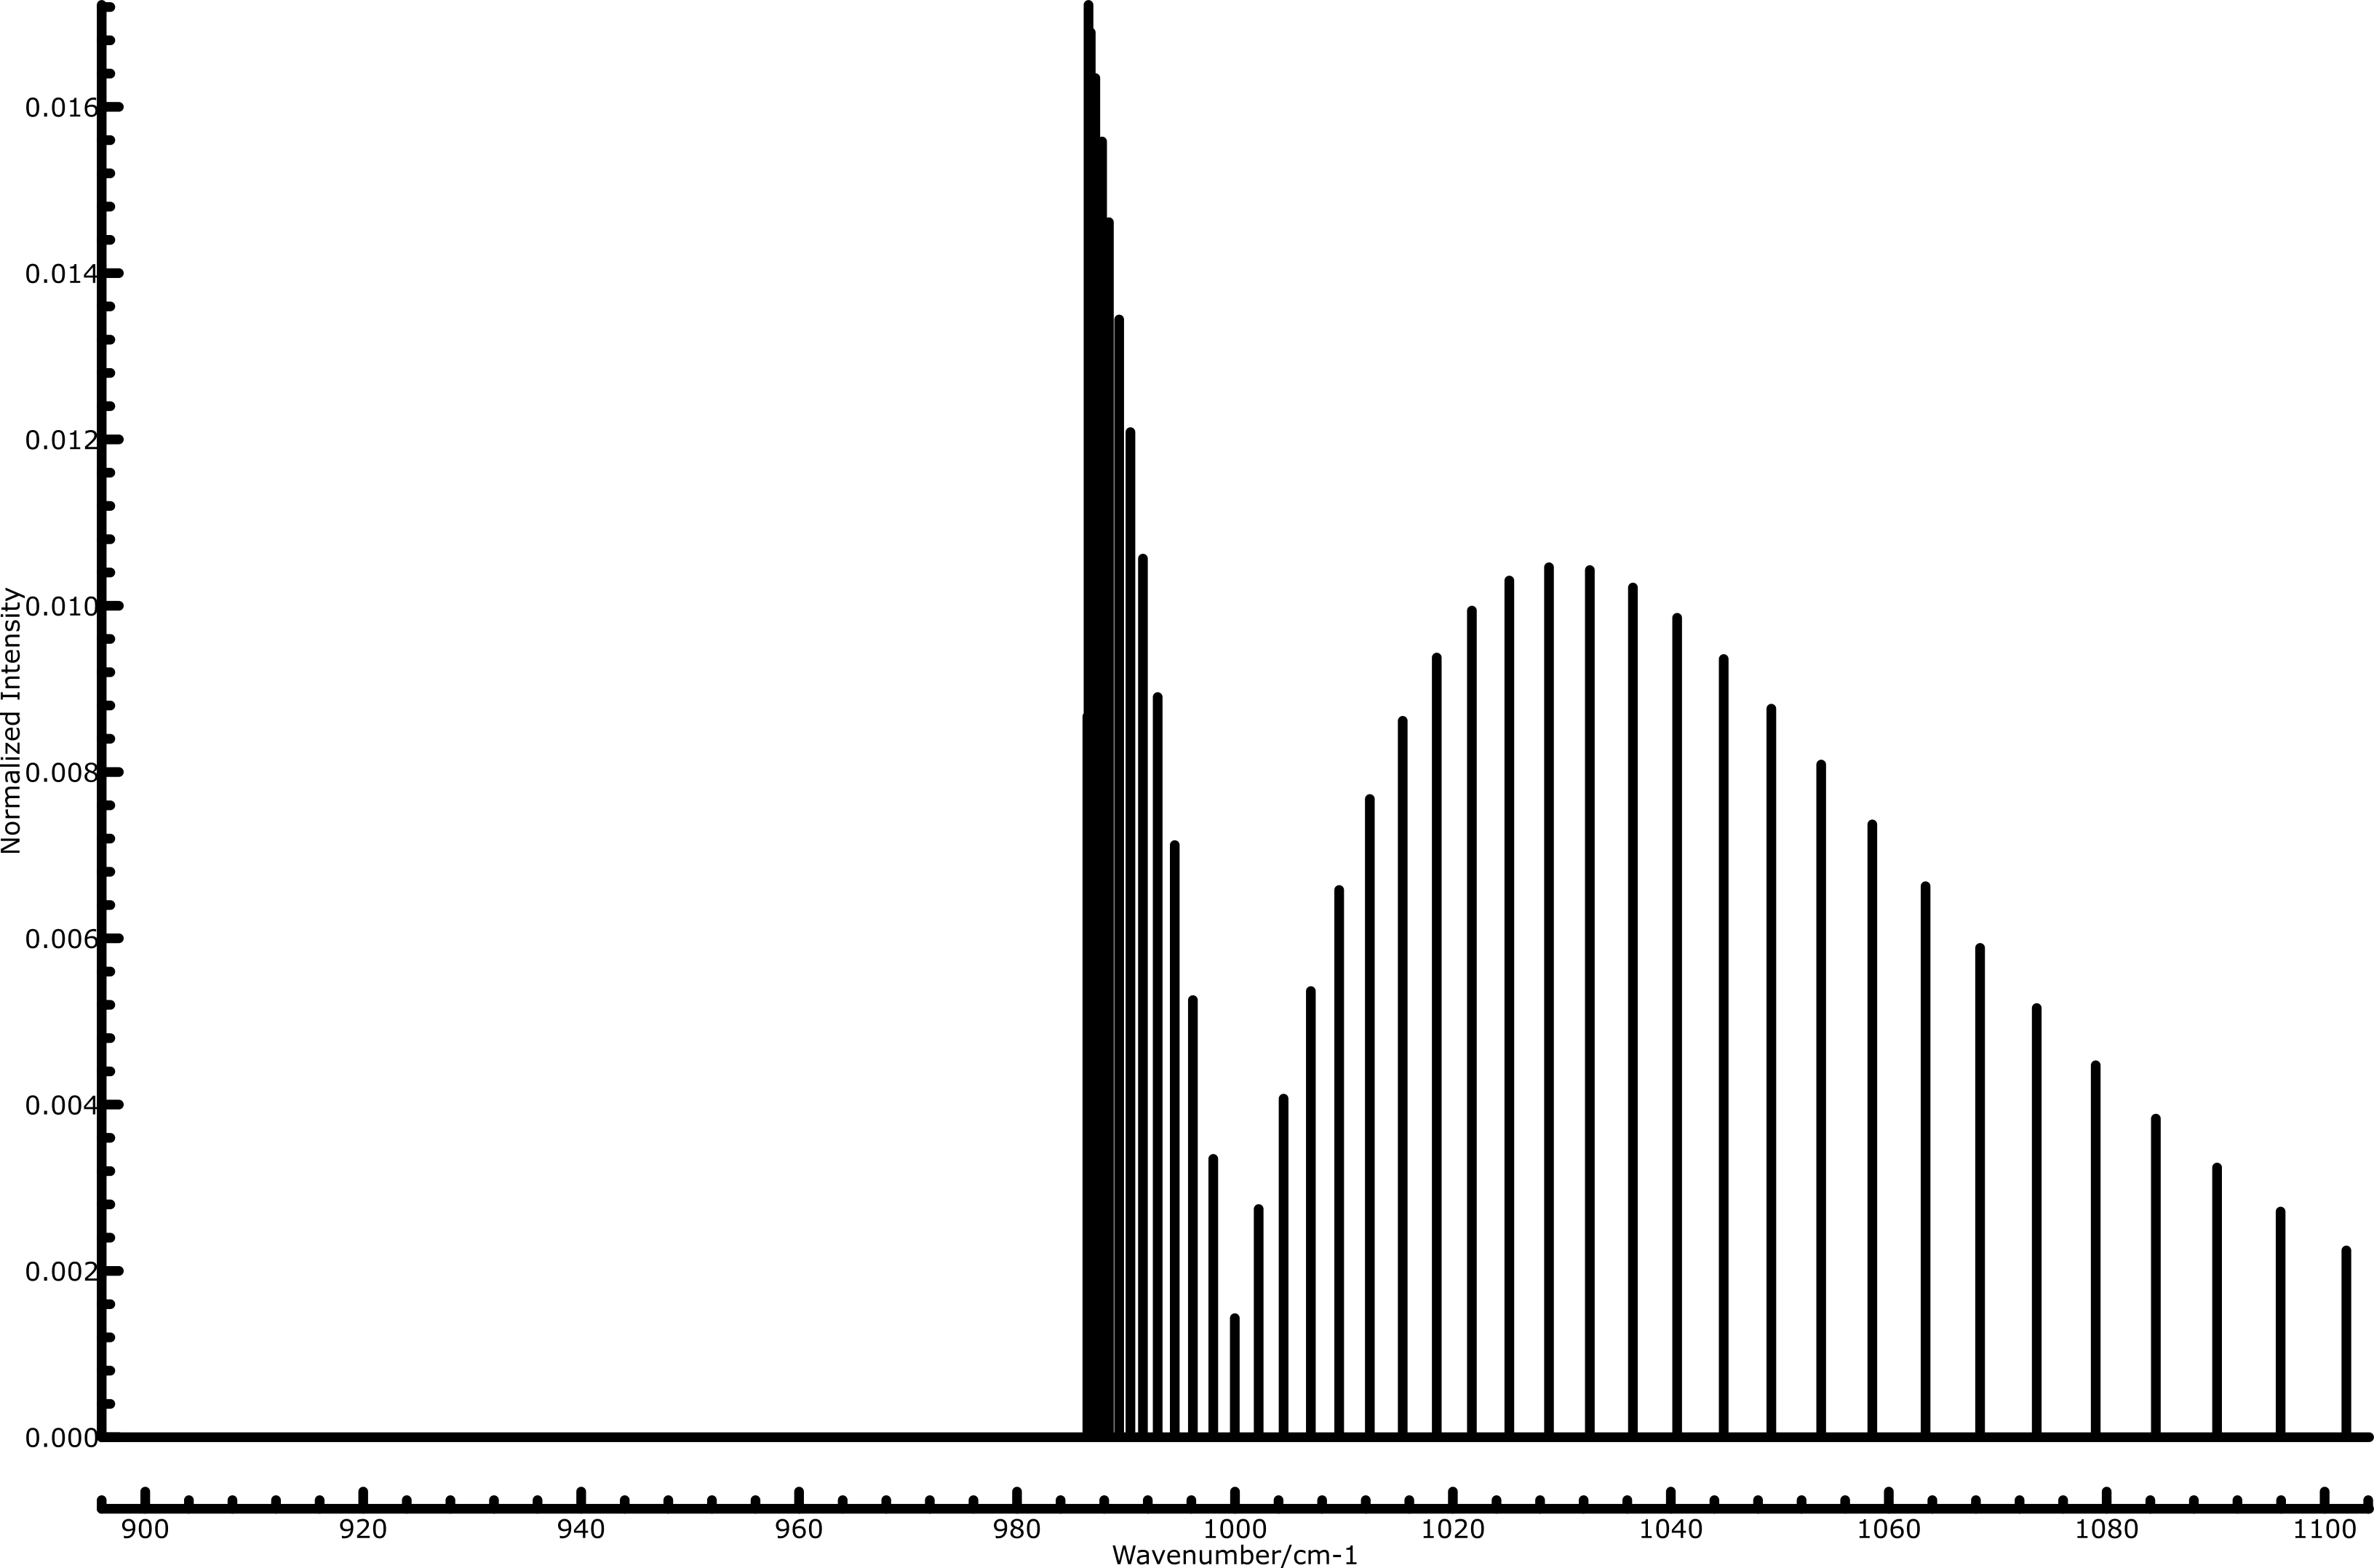
\includegraphics[width=\linewidth]	  					{figures/B108.png}
			\end{figure}
				\centering(B = 1.08) \\
		\end{minipage}
	\end{minipage}
\end{center}
\begin{center}
	\begin{minipage}{\linewidth}
		\begin{minipage}{0.5\linewidth}
			\begin{figure}[H]
				\centering 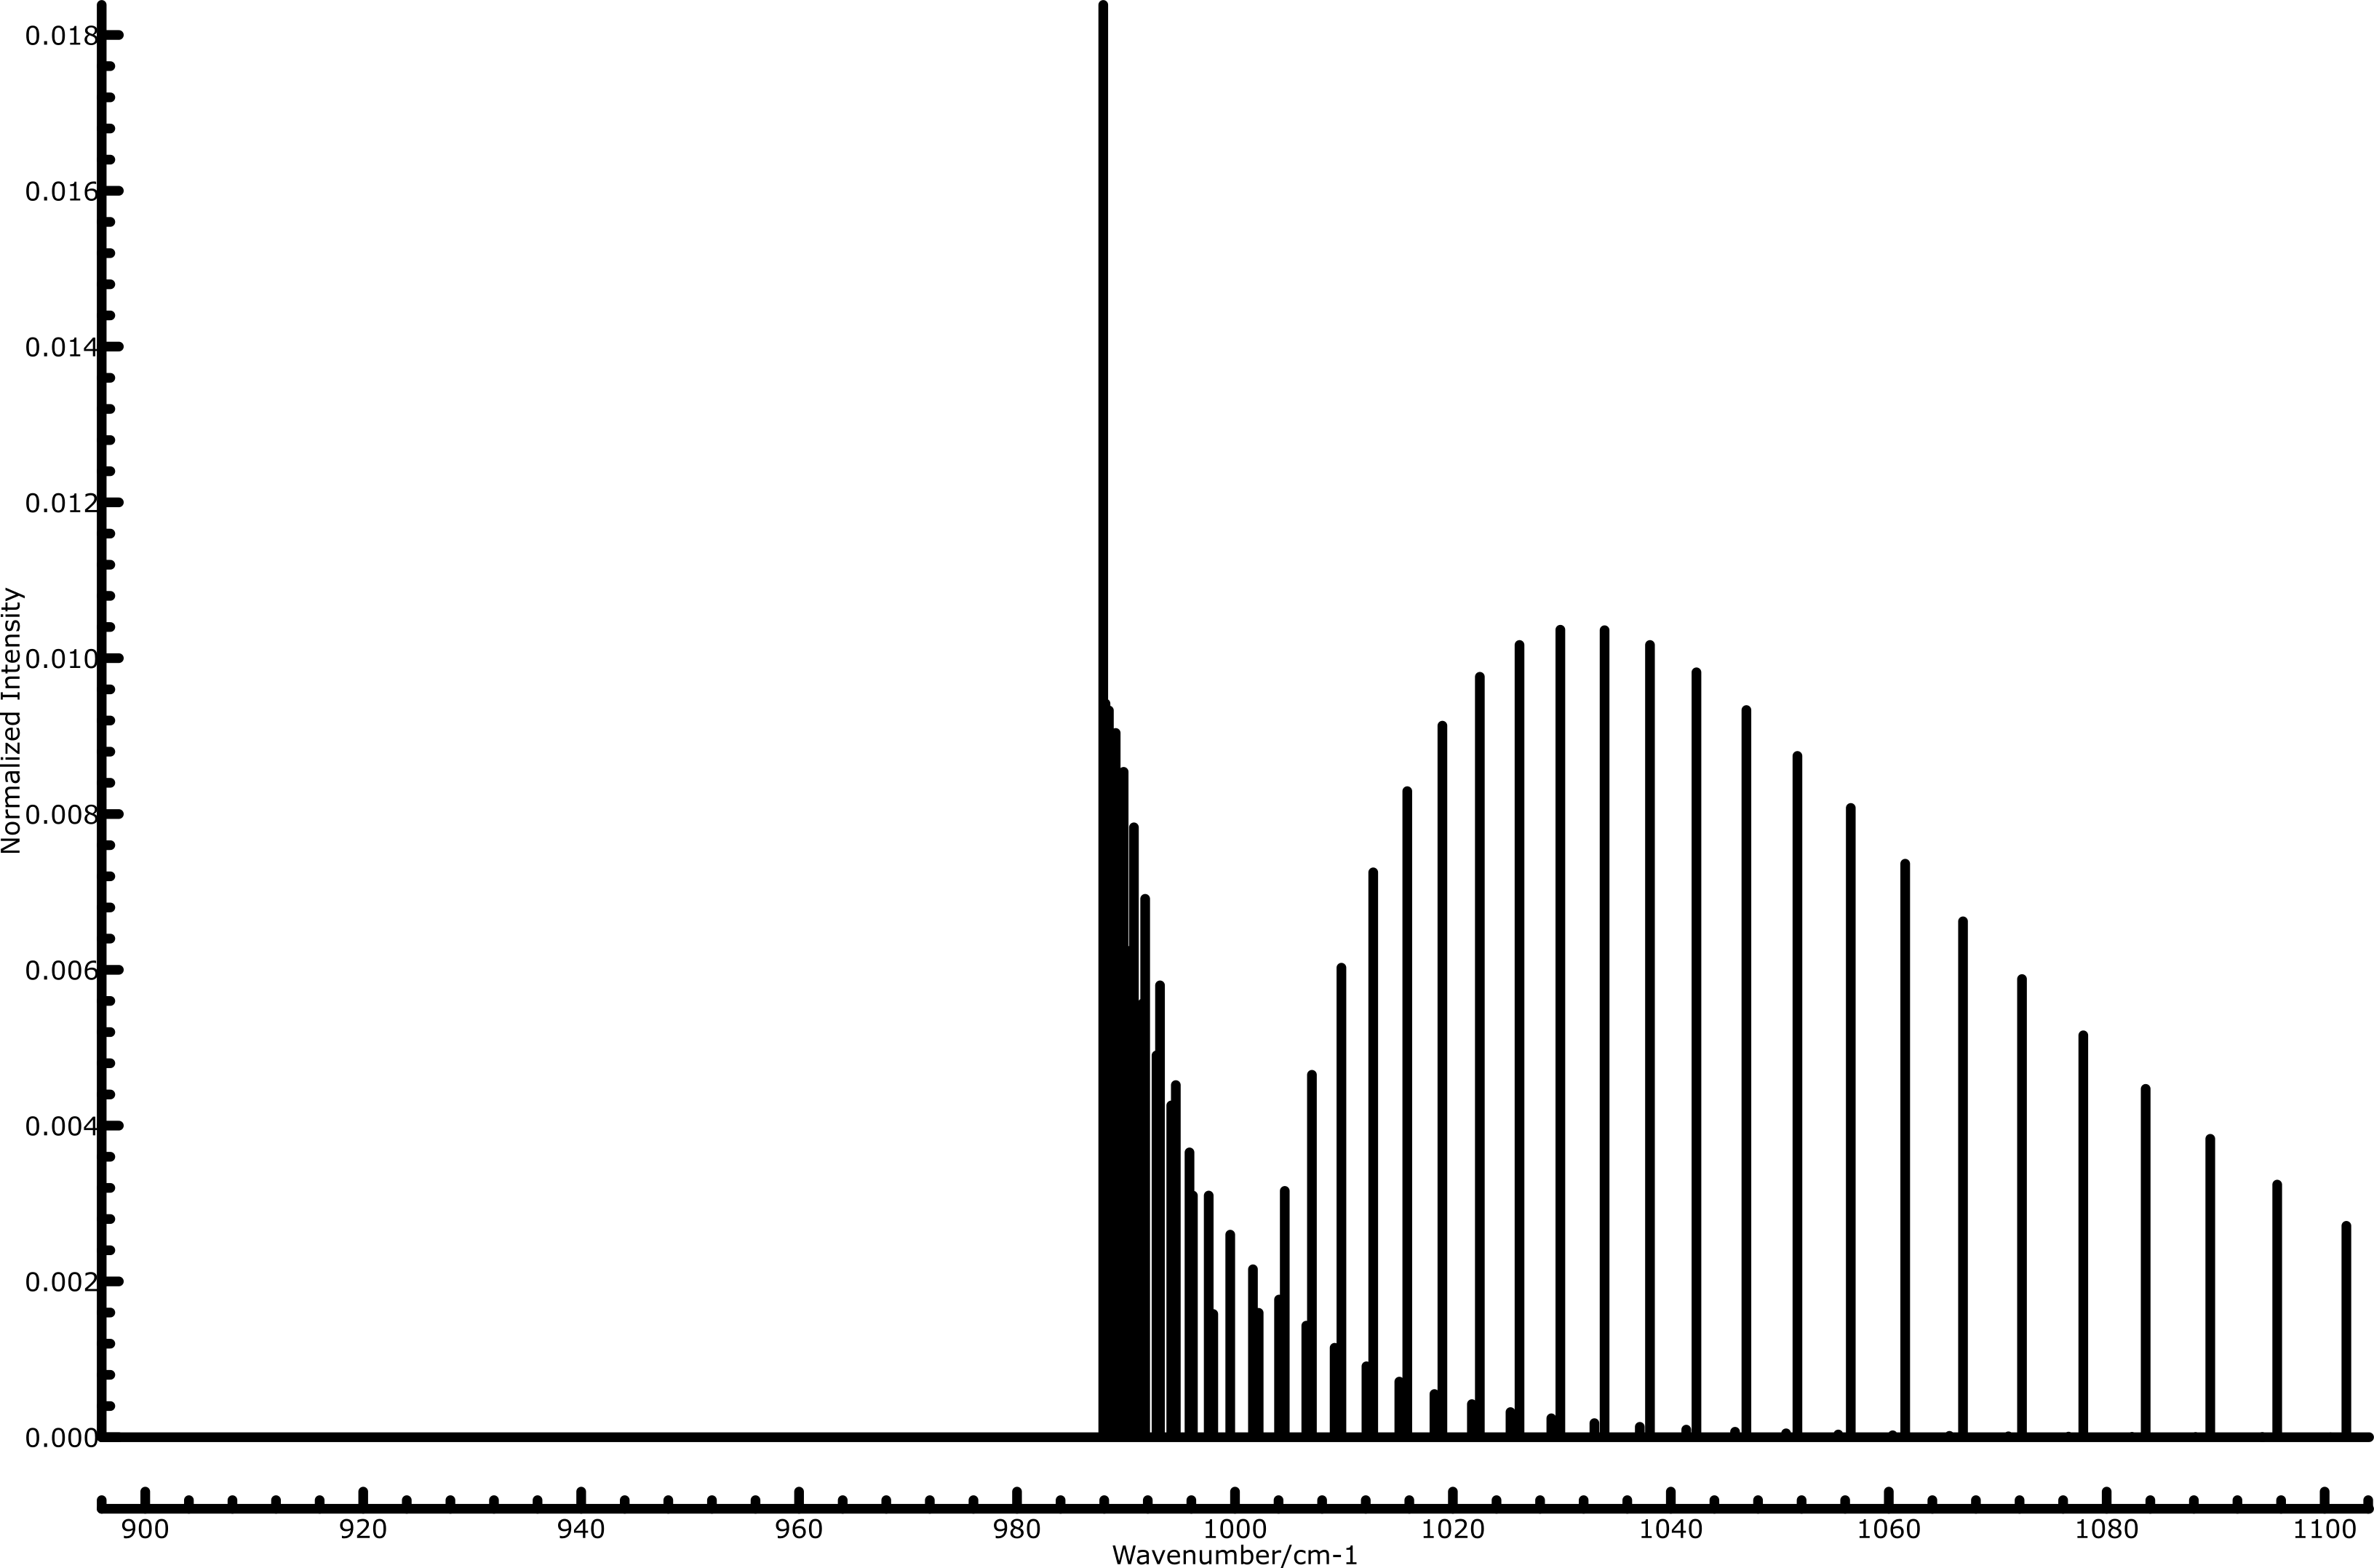
\includegraphics[width=\linewidth] 						{figures/B109.png}
			\end{figure} 
				\centering(B = 1.09) \\
		\end{minipage}
		\begin{minipage}{0.5\linewidth}
		   \begin{figure}[H]
				\centering 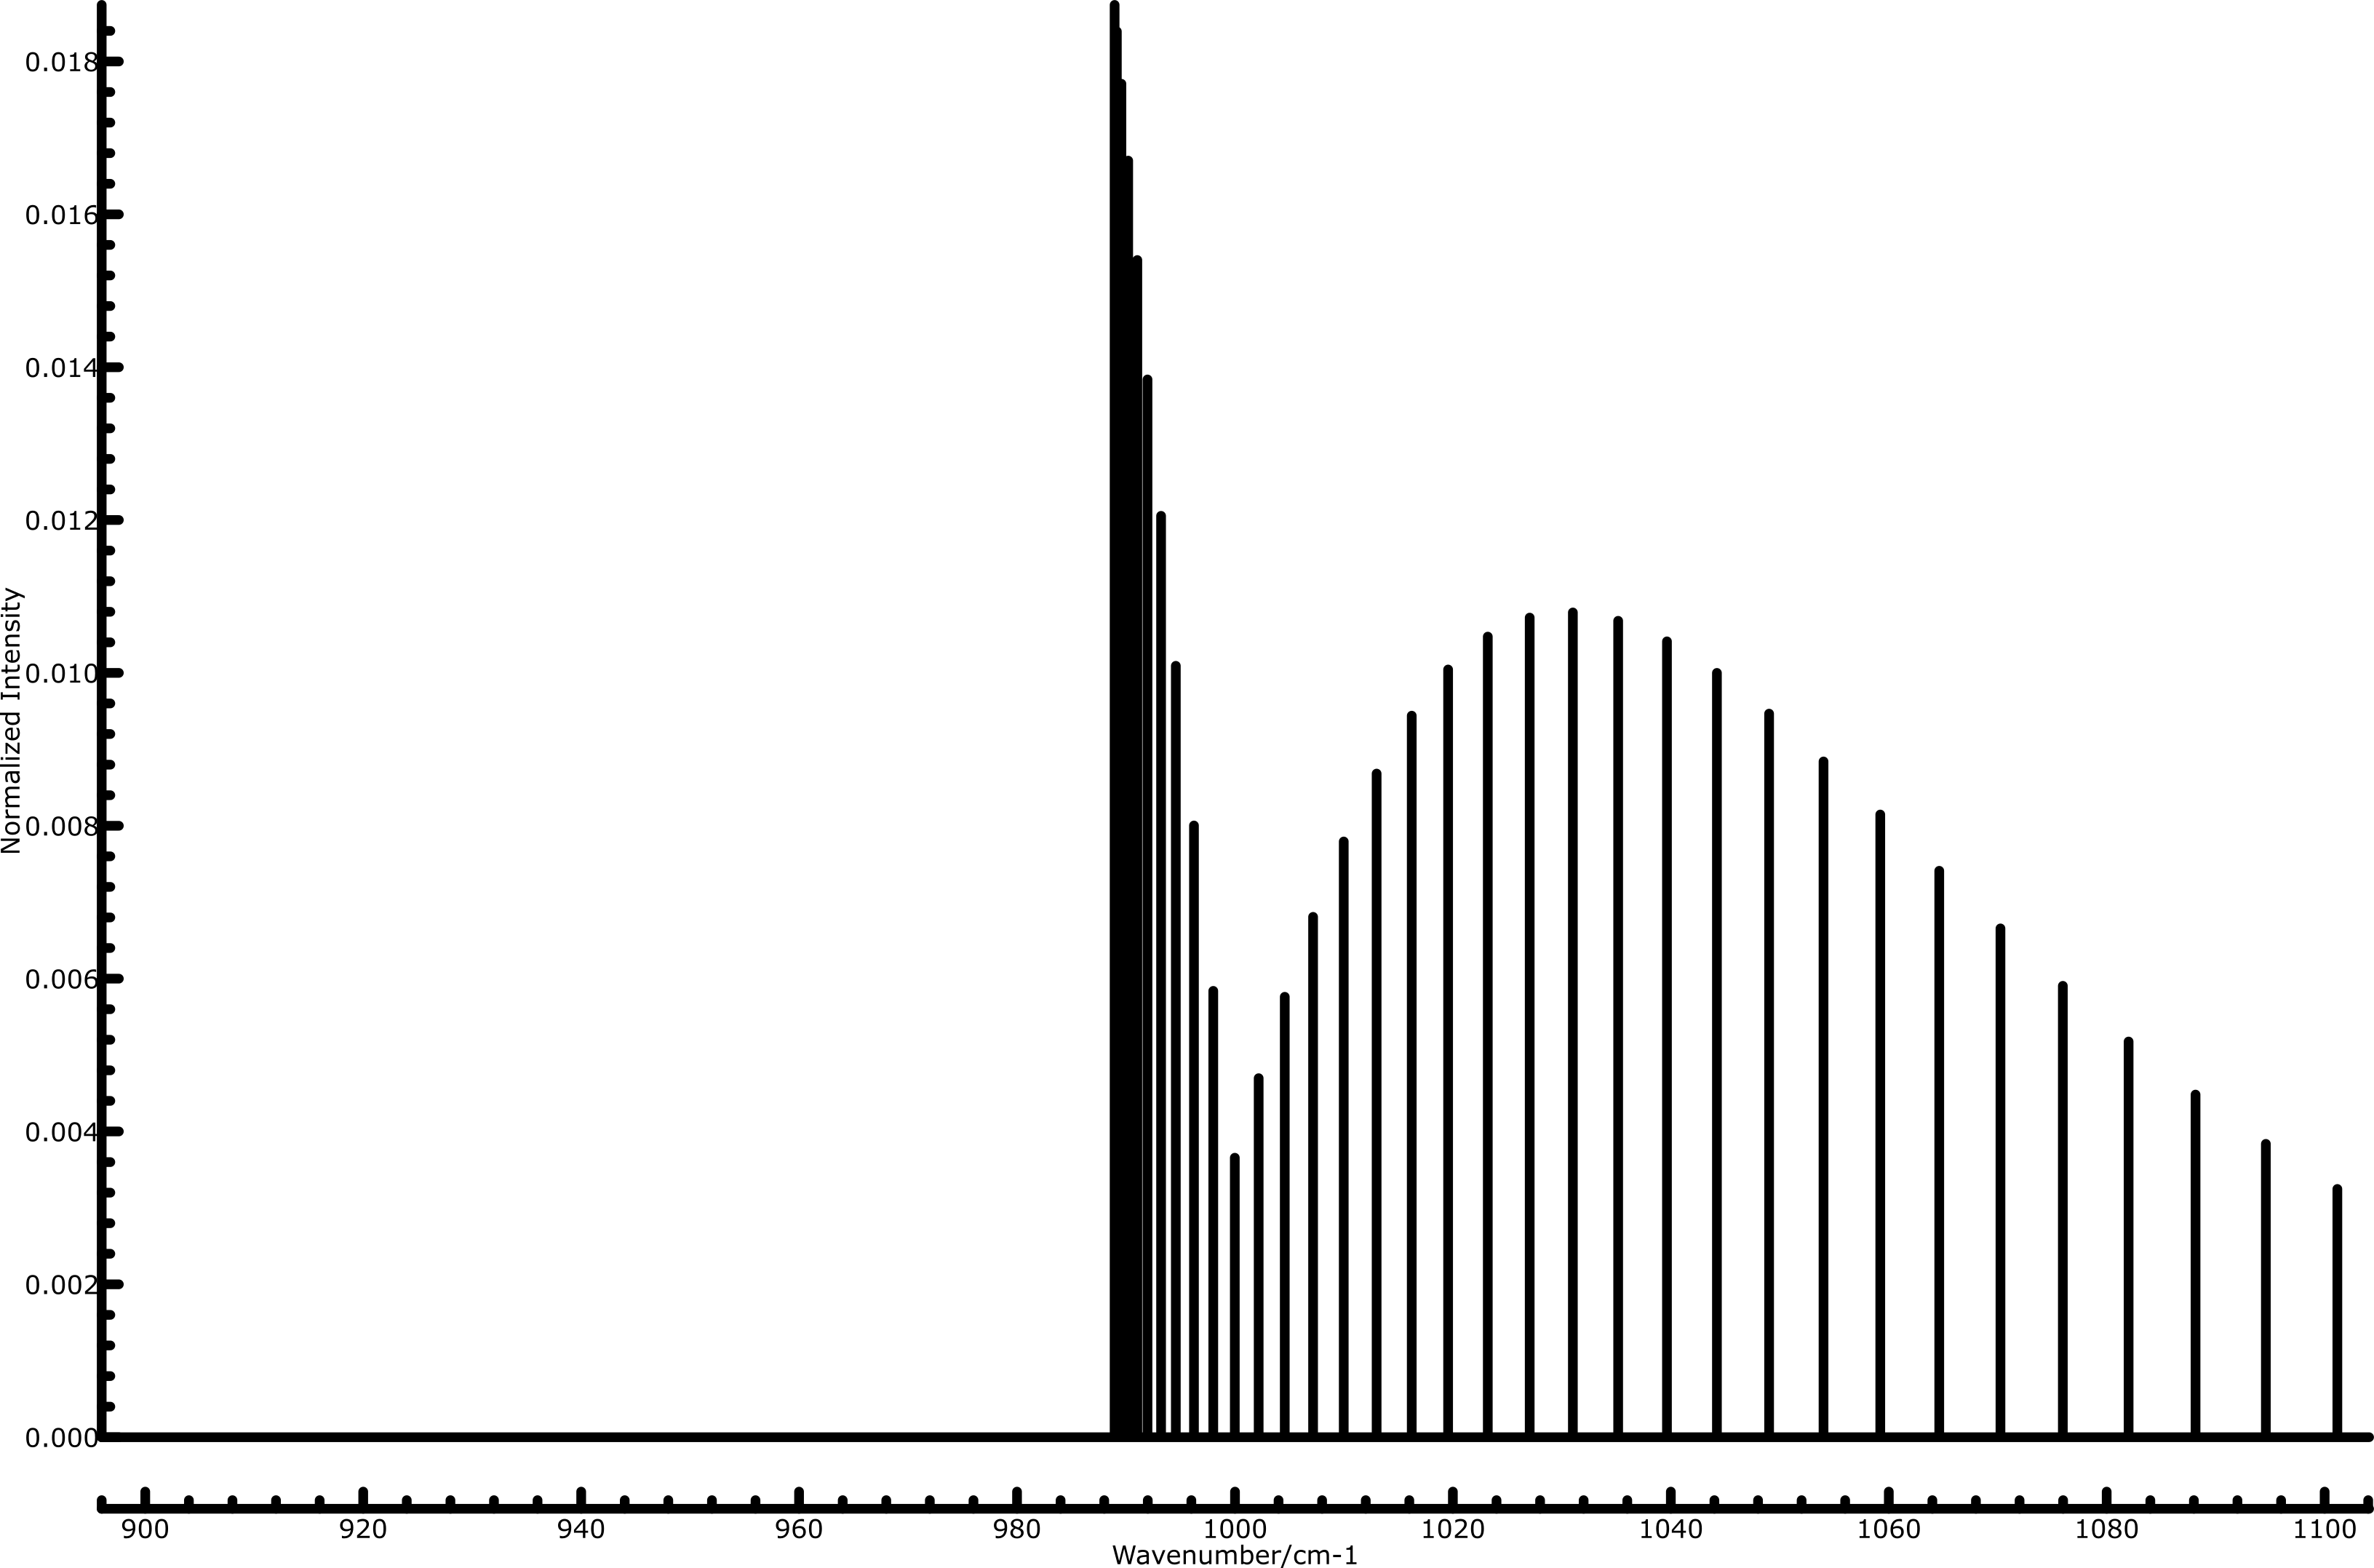
\includegraphics[width=\linewidth]	  					{figures/B110.png}
			\end{figure}
				\centering(B = 1.1) \\
		\end{minipage}
	\end{minipage}
\end{center}

\end{document}